%
% Szakdolgozat minta az Eszterházy Károly Egyetem
% matematika illetve informatika szakos hallgatóinak.
%

\documentclass[
% opciók nélkül: egyoldalas nyomtatás, elektronikus verzió
% twoside,     % kétoldalas nyomtatás
% tocnopagenum,% oldalszámozás a tartalomjegyzék után kezdődik
]{thesis-ekf}
\usepackage[T1]{fontenc}
\PassOptionsToPackage{defaults=hu-min}{magyar.ldf}
\usepackage[magyar]{babel}
\usepackage{mathtools,amssymb,amsthm}
\usepackage{enumitem}
\usepackage{array}
\usepackage{longtable}
\usepackage{graphicx}
\newcolumntype{L}{>{\centering\arraybackslash}m{7.5cm}}
\usepackage{listings}
\def\lstlistingname{kód}
\usepackage{xcolor}
\lstset{language=[sharp]C,basicstyle=\footnotesize,
	keywordstyle=\bfseries\color{blue},numbers=left,
	frame=tRBl,frameround=tftt,breaklines=true,morekeywords={async}}
\footnotestyle{rule=fourth}

\newtheorem{tetel}{Tétel}[chapter]
\theoremstyle{definition}
\newtheorem{definicio}[tetel]{Definíció}
\theoremstyle{remark}
\newtheorem{megjegyzes}[tetel]{Megjegyzés}

\begin{document}
\institute{Matematikai és Informatikai Intézet}
\title{Iktató program készítése szociális intézmény részére}
\author{Pekár Mihály\\Programtervező informatikus BSc}
\supervisor{Balla Tamás\\Tanársegéd}
\city{Eger}
\date{2020}
\maketitle
\tableofcontents
\chapter{Bevezetés}

Szakdolgozatom témájaként a munkám során mindennap előforduló iratkezelési problémát szeretném megoldani. Az intézmények a nyomon követhető háttérmunka nélkül nem képesek működni, ezért a napi munka során keletkezett dokumentáció szakszerű kezelése és iktatása nélkülözhetetlen. Mivel minden közfeladatot ellátó szerv, intézmény, vállalat más és más tevékenységet végez, ezért számukra elengedhetetlen a pontos, precíz iratkezelés, amit szabályozott és rendszeres ügyviteli munkával érhetnek el.

2018 évében egyes állami fenntartásban lévő szociális szférában működő szervezeteket egyházi tulajdonba kerültek. Ennek következményében a Szociális- és Gyermekvédelmi Főigazgatóság fennhatósága alatt álló Békés Megyei Körös-menti Szociális Centrum szarvasi telephelye a Magyarországi Evangélikus Egyház szarvasi diakóniájának részévé vált. Mivel egy időben több telephellyel is bővült, ezért szükségessé vált az ügyviteli, leltározási és nyilvántartó rendszereinek felülvizsgálata. Az eddig 50 fővel működő diakónia létszámához elegendő volt az Excel használata, viszont a megtöbbszöröződött létszámmal a dokumentumok átláthatatlanabbak, kezelhetetlenebbek lettek és egyre több problémát okoztak az elszámolásokban, kimutatásokban, zárásokban. Ekkor keresett meg a gazdasági vezető olyan céllal, hogy e munkafolyamatokat rendszerezzük, szabályozzuk és egyszerűsítsük le szoftverek segítségével. Programozói feladataim között szerepelt munkaruha, leltár és telephelyek ételadag megrendeléseit nyilvántartó rendszerek fejlesztése. Számomra ez egy jó lehetőséget adott, hogy a tanulmányaim során szerzett programozói tudást gyakorolhassam. Megragadtam az alkalmat és minden egyes programhoz más és más programozási nyelvet alkalmaztam. Sok segítséget nyújtott számomra, hogy ezek nagy részét már lehetőségem volt kurzus keretei között megtanulni az egyetemen. Például a munkaruha nyilvántartóhoz HTML, JavaScript és CSS-t, keretrendszernek node.js és bootstrap-t választottam, ezek nagyban megkönnyítették a fejlesztést. A leltár programhoz a java Spring-keretrendszerét alkalmaztam, de kipróbáltam az Excel-ben a VBA programozási nyelvet is.

Ezen programok fejlesztése után jutottunk el az iktatáshoz, amelyet ugyanúgy Excel-ben végeztek a kollégák. A vezető mindenképpen le szerette volna cserélni ezeket a munkafüzeteket, mert teljesen alkalmatlanokká váltak a megnövekedett mennyiségű iratok kezeléséhez. Arra jutottunk, hogy ezeket a munkafolyamatokat egy erre fejlesztett programban kellene végezni. A várható pozitív hatások, úgymint az egyszerűbb áttekinthetőség, a gyorsaság és a költséghatékonyság megerősített minket a szoftver létrehozásában. Arról még említést se tettünk, hogy egyre több irat érkezik valamilyen elektronikus formában és ezeknek a tárolása, megőrzése nem egyszerű. Első és legfontosabb vágy, kritérium az volt, hogy ebben a programban nyomon követhessék az összes telephelyen keletkező iktatást, továbbá az is fontos követelmény, hogy a dokumentumok könnyen és pontosan visszakereshetőek legyenek.

Így a dolgozatom célja munkáltatóm ügyviteli rendszerének összehangolása, átszervezése, iktatásának központosítása és digitalizálása. Azért hangsúlyos ez a terület ebben az intézményben, mert az itt folyó szociális és ápolói munka során számos egyéb hivatalos szervvel kerülünk kapcsolatba, ami megköveteli a naprakész, pontos és folyamatában követhető iratkezelést.

A dolgozatom következő fejezetében bemutatom a szoftver fejlesztés megkezdéséhez szükséges specifikációkat amiket a félreértések elkerülése érdekében készítettem. A harmadik fejezetben említést teszek a felhasznált technológiákról, ami magába foglalja a kliens oldali Caliburn.Micro MVVM keretrendszert, a szerver és kliens szétválasztását lehetővé tevő gRPC-ről. A negyedik fejezet a kliens és szerver oldali implementálásokról illetve azok fontosabb összetevőiről fog szólni, valamint az adatbázis kialakításáról. Végül az összefoglalás előtti fejezet a kimaradt és a visszajelzések alapján megfogalmazódott fejlesztésekről szól. 

\chapter{Követelmény specifikáció}
\section{Fogalomtár\cite{rendelet}}
\begin{itemize}[leftmargin=0pt]
 	\item[] \textbf{iktatókönyv:} Olyan nem selejtezhető, hitelesített iratkezelési segédeszköz, amelyben az iratok iktatása történik: a be- és kimenő iratok nyilvántartásba vétele, iktatószámmal történő ellátása, dátum és partner megjelölésével.
	\item[] \textbf{user:}  Az a személy, aki az adott funkció használatára jogosult és a funkció működtetése során számára ismertté váló vagy módosítható adatokhoz rendelkezik a betekintési vagy módosítási jogosultsággal.
	\item[] \textbf{admin:} Az a személy, akik a user jogosultságnál magasabb hozzáférési szinttel rendelkeznek.
	\item[] \textbf{rendszergazda:} Az a személy, aki az iktatóprogram telepítésével, karbantartásával, rendszernapló gondozásával, valamint a szerver működésének ellenőrzésével foglalkozik.
	\item[] \textbf{szerver: }Olyan nagyteljesítményű számítógép vagy szoftver, ami a más számítógépek számára a rajta tárolt vagy előállított adatok felhasználását a szerver, hardver erőforrásainak kihasználását, illetve más szolgáltatások elérését teszi lehetővé.
	\item[] \textbf{adatbázis: }Azonos minőségű többnyire strukturált adatok összessége, amelyet egy tárolására, lekérdezésére és szerkesztésére alkalmas szoftvereszköz kezel.
	\item[] \textbf{iktatás: }Iratnyilvántartás alapvető része, amelynek során a beérkező iratot, illetve a keletkezett iratot iktatószámmal látják el.
	\item[] \textbf{partner: }A szervezet azon résztvevői, akik felé hivatalos iratok készülnek. Ez lehet cég, magánszemély vagy más hatóság.
	\item[] \textbf{partnerügyintéző: }Az a személy, aki a partnernél hivatalos irattal foglalkozik.
	\item[] \textbf{telephely: }Az intézmény különböző földrajzi helyeken elhelyezkedő egységei.
	\item[] \textbf{jelleg: }Az iktatott anyag formája. Lehet fax, e-mail, levél, munkaügyi irat stb.
	\item[] \textbf{iktatásicsoport: }Ügyirat besorolását, osztályozását lehetővé tevő zárt adatkészlet, amelyhez az adott szervnél ügyirat hozzárendelhető.
	\item[] \textbf{ügyintéző: }Az a személy, aki az ügyirat nyilvántartásba vételével foglalkozik.
	\item[] \textbf{irány: }Azon jellemző, amely megmutatja, hogy az intézmény felé érkezett vagy általa küldött  az irat.
	\item[] \textbf{törzsadat: }Azon adatok összessége, melyekből az iktatás összeáll.
	\item[] \textbf{logolás: }Olyan adatok rendezett összessége, amely az események rekonstruálására alkalmas, részletességben tárol információt az iratkezelési eseményekről és egyéb tevékenységekről.
	\item[] \textbf{irat: }A köziratokról, a közlevéltárakról és magánlevéltári anyag védelméről szóló 1995. évi LXVI. törvény 3.§ c pontja szerinti adat együttes.
	\item[] \textbf{előzményezés: }Az iratkezelési folyamat azon művelete, amely során megállapításra kerül, hogy az új irat egy már meglévő ügyirattal kapcsolatban áll-e, vagy az új iratot új ügy első irataként kell-e nyilvántartásba venni.
	\item[] \textbf{hivatkozási szám: }A beérkezett irat iktatási száma.
	\item[] \textbf{jogosultság:  }Egy adott művelet elvégzésének lehetősége az iktatóprogramban, egy adott személyre vagy rendszerelemre vonatkozóan, szerepkör hozzárendelése.
\end{itemize}
\section{Jelenlegi helyzet leírása}
Minden hivatalos iratokkal foglalkozó kollégánál van egy Excel tábla, amit iktatásra használ. Ebben a táblában iktatja a hozzá beérkező, illetve az általa elkészített ügyiratokat. Hátrányai ennek a helyzetnek, hogy az iktatások állandósága sérül, azaz egy-egy irat kaphat olyan számot, ami már foglalt. Mivel vannak, olyan esetek, amelyek több munkacsoportot is érintenek, az adott irattal előfordulhat, hogy többször vagy egyszer sem iktatnak le. Az iktatásokhoz nem lehet előzményezést rendelni. Az egységek nem látják egységesen az iktatási anyagaikat, így egymás segítségére szorulnak. Az iktatott dokumentumokat csak több perces keresés árán tudják megtalálni. 
Excel hibái a jelenlegi helyzetre:
\begin{enumerate}[leftmargin=0pt]
	\item A legtöbb embernek nincs kellő ismerete
	
A legtöbb dolgozó zavarónak és félelmetesnek találják az Excelt, ezért meg sem próbálják megtanulni a használatát. Leginkább ez azon dolgozókra igaz, akik nem rendelkeznek sok tapasztalattal az Excelről. Ez nálunk sincs másképp, hasonló problémákba ütközök nap, mint nap a kollégáim körében. Ha valaki kap egy feladatot, amit Excelben kell elvégeznie a legapróbb nehézségnél is segítséget kér.
   \item A fontos adat eltűnik
  
Mivel az összes adatot látjuk egyszerre, ezért nagyon nehéz átnézni úgy, hogy felfedezzük melyik adat fontos és melyik nem.\cite{excel} Sokszor tapasztalom azt a kollégák körében, hogy a használt Excel dokumentumokat több percig is nézik, hogy megtalálják a keresett adatot, amire kíváncsiak voltak. Természetesen lehet használni színezéseket is, de e módszerek használata egy idő után növelik az átláthatatlanságát.\cite{excel} Továbbá a nem egységesen használt színkezelés csak bonyolítják az értelmezését. 
	\item Nyomonkövetés
	
Sok esetben előfordult, hogy a dolgozók egymás adatait véletlenül törölték, módosították. Mivel a munkafüzetet nem arra tervezték, hogy eltárolja a változásokat, ezért ha egy adatot módosítunk vagy törlünk, azt csak mentésből tudjuk visszaállítani. Ezeknek a manipulációknak a visszakövetése nem lehetséges. 
	\item Megosztás
	
A felhőalapú technológiák manapság már megkönnyítik a dokumentum megosztást a dolgozók között, de még mindig nem a legjobb megoldás. Mivel annak a lehetősége, hogy az adatot kitörlik vagy megváltoztatják, a munkafüzetet ritkán tesszük elérhetővé mások számára valós időben. \cite{excel}
	\item Az adatkezelési szabályok betartása 
	
Az Excelben nem lehet az iktatószámokat nyomon követni és azok konzisztenciáját megőrizni. Könnyen el lehet rontani az iktatószám felépítését. Több telephely iktatásának tárolása a munkafüzeten komplikációt okoz, illetve nincs kontroll az iktatások felvitelében, így bárki bármikor ütközhet. A dokumentumkezelés is nehézséges, az iktatásokhoz külső link formájában hozzáadhatjuk a dokumentumot, viszont ha ezek az adatok más helyre kerülnek, akkor az összes csatolt linket módosítani kellene. 
	\item Nem célszoftver
	
Ezt a programot nyilván nem iktatás, ügyiratkezelés folyamataira tervezték, az adatmennyiség  és ezen folyamatok bonyolultságának  növekedésének köszönhetően a szoftvernek a használata egyre kellemetlenebbé válik. 
	\item Jogosultság

A felhasználók kezelésére és azoknak a jogosultságának szabályozására sincs lehetőség. Így bármilyen adaton bárki tud módosítást végezni. Már pedig ez számunkra nagyon fontos funkció, hogy ezeket a folyamatokat felhasználó szinten tudjuk befolyásolni, hogy az adatok biztonságban legyenek. 

\end{enumerate}

\section{Vágyálom rendszer}
Egy olyan központosított iktatás létrehozása, ahol a személyenkénti gondolkodásmódot elhagyhatjuk. A gazdasági csoport vezetője szeretné látni az összes telephely iktatását, mivel a jelenlegi helyzetben ez nem megoldott. Feleljen meg az iratkezelésre vonatkozó jogszabályoknak és az intézményi ügyiratkezelési szabályzatnak. A legfőbb cél, hogy az iratkezelés legyen szakszerű, gyors, gazdaságos és naprakész.

Tudjon felhasználókat kezelni a program, azaz legyen lehetőség a userek hozzáadására, módosítására és inaktívvá tételére. Két jogosultsági szint legyen, sima felhasználó és admin. A jelszavakat az adatbázisban titkosítva tárolja. El lehessen különíteni telephelyeket, illetve legyen olyan lehetőség is, hogy egyes felhasználókhoz több telephely is tartozzon vagy mind.

Az iktatás összeállítása egyszerű és könnyen kezelhető, valamint az iktatószám azonnal olvasható legyen. Ne kelljen ügyelni arra, hogy ki és mikor iktat, a program automatikusan generálja a megadott adatokból az iktatószámot. Ez úgy generálódjon, hogy vegye figyelembe a felhasználó által felvitt adatokat és az aktív évet. Minta az iktatószámra: B-M/R/2/2020, az első betű reprezentálja az iktatásnak az irányát, a kötőjel utáni rész az iktatási csoportot jelölje, ami maximum 3 karakter hosszúságú lehet.  Az „R” betű jelöli a telephely kezdőbetűjét, ebből is tudni fogjuk, hogy az iktatás melyik telephelyhez tartozik. Ezután következik a sorszám, ami a soron következő iktatást jelöli a telephelyen. Az utolsó szakasz az aktív évet jelölje. Illetve szeretnénk egy olyan eljárást is, ahol a felhasználó kiválaszthatja az iktatás előzményét. Ezáltal az iktatószámot oly módon befolyásolja, hogy a korábban iktatott számnak soron következő alszámát generálja le (előzményezés). Például: B-M/R/2-1-2/2020. Évenként elkülöníthetők és lezárhatóak legyenek az iktatások. Irányuk lehet bejövő és kimenő jellegű.

Törzsadatokat egy menüpontban legyen lehetőség kezelni. A felhasználók számára legyen elérhető partner, ügyintéző, partner ügyintézője, jelleg adatok kezelése. Adminnak ezeken kívül legyen még lehetősége a csoport, telephely, felhasználók, év zárás/nyitás módosítására, felvitelére.  Viszont a felhasználók jelszavát csak a rendszergazda módosíthatja.

A dokumentumot gyorsan és egyszerűen fel lehessen tölteni az iktatásokhoz. Ezek jellege Word, Excel, PDF. Könnyen lehessen keresni a felvitt adatok között. Egyes iktatásokhoz több dokumentum is csatolható legyen. Ezeknek a dokumentumoknak a megtekintésére, letöltésére és törlésére legyen lehetőség. 

A rendszergazdának legyen szerveren kezelő felülete, ahol az adatbázist, felhasználókat és a naplózást könnyen tudja kezelni. Itt legyen meg az a lehetősége, ahol a felhasználók jelszavát módosíthatja.

Jó lenne az egyházi jelleg megjelenése a programban. Például a főoldal tartalmazhatná a napi igét, illetve az evangélikus egyház jelképe, azaz a Luther-rózsa is megjelenhetne.
\section{A rendszerre vonatkozó pályázat, törvények, rendeletek, szabványok és ajánlások felsorolása}
Az iratkezelés menetét az applikációban alapvetően 2 törvény határozza meg, ezek a jelenleg hatályos, többször módosított, a levéltári törvény a köziratokról, a közlevéltárakról és a magánlevéltári anyag védelméről szóló \textbf{1995. évi LXVI. törvény},\cite{torveny} valamint a közfeladatot ellátó szervek iratkezelésének általános követelményeiről szóló \textbf{335/2005.(XII: 29.) Korm. rendelet}\cite{rendelet}. 

A kormányrendeletben szereplő 6.§-ban foglalt egyes pontjai határozzák meg a program működését legfőképpen. Ezek a pontok magukba foglalják, hogy 
\begin{itemize}
	\item a szervezethez érkezett, ott keletkező, illetve onnan továbbított irat azonosítható, fellelési helye, útja követhető, ellenőrizhető és visszakereshető legyen;
	\item az irat tartalma csak az arra jogosult számára legyen megismerhető;
	\item az irat kezeléséért fennálló személyi felelősség egyértelműen megállapítható legyen.
\end{itemize}

A törvény a 9.§ -ban foglaltak alapján a program, az intézményhez érkezett és az általa készített iratokat az érkezés, illetve a keletkezés időpontját eltárolja, azaz nyilvántartásba veszi. Valamint a keletkező, nem selejtezhető iratoknak tartós megőrzését kell lehetővé tennie.

Mivel az \textbf{intézmény ügyiratkezelés szabályzata} ezen törvények előírásai alapján készült tehát szabályozza az iratok biztonságos kezelési módját, szakszerű iktatását és megőrzését. Ide tartozik minden olyan feladat, ami az iratok átvételéhez, érkeztetéséhez, elosztásához, nyilvántartásba vételéhez, irattárazásához. Így a program írásakor figyelembe kellett venni, hogy az iktatási csoportok elkülöníthető betűjeleket kapjanak, valamint külön telephelyekre vonatkozó választási lehetőség legyen. Ezen felül a telephelyeket és ügyirati csoportokat ez a szabályzat határozza meg. 

\section{Követelmény lista}
A fent említett igények alapján állítottuk össze a követelmény listát, ami megfogalmazza, hogy egyes verzió számú program részek már milyen tudással bírjanak.
\begin{longtable}{|c|c|c|L|}

	\hline 
	ID & Név & V. & Kifejtés \\ 
	\hline 
	1 & Bejelentkezés  & 0.1 &  \multicolumn{1}{m{7.5cm}|}{
		Legyen egy szép és egyszerű bejelentkezési felület, ahol a felhasználó nevet el lehessen menteni, de csak akkor, ha szeretné a user. A felhasználók jelszavát a rendszergazda se tudja visszanézni, viszont módosítani csak ő tudja. 
	}\\ 
	\hline 
	2 & Főoldal és ige & 0.2 & \multicolumn{1}{m{7.5cm}|}{A belépés után jelenjen meg az üdvözlő felület. Ahol megtalálható az egyház szimbóluma, és a napi ige.} \\ 
	\hline 
	3 & Törzsadatok kezelése & 0.3 &\multicolumn{1}{m{7.5cm}|}{ Egy helyen lehessen kezelni a törzset. Mindegyik törzshöz legyen lehetőség hozzáadni, törölni és módosítani. Minden telephelyhez külön törzs adatbázis tartozzon, ne keveredjen a többi telephellyel. A felhasználó jogosultsággal rendelkező munkatárs ne tudjon iktatási csoportot, telephelyet, felhasználót és évet kezelni. }\\ 
	\hline 
	4 & Iktatás kezelhetősége & 0.4 & \multicolumn{1}{m{7.5cm}|}{Az iktatáshoz tartozó információk egy legördülő menüben kiválaszthatók legyenek(ügyintéző, jelleg, csoport, stb\dots). A tárgynak és hivatkozási számnak legyen külön beviteli mezője, csak aktuális évre lehessen iktatni. Előzményezési lehetőség is legyen. Az iktatásokat törölni csak admin jogosultsággal. Az iktatások bárki által módosíthatók, de csak azokat az információkat, amik nem befolyásolják az iktatószámot. Két dátum, érkezett és határidő lehessen megjegyzést fűzni az iktatáshoz. A hivatkozási szám, megjegyzés és a partnerügyintézőn kívül minden mezőt kötelező kitölteni.} \\ 
	\hline 
	5 & Dokumentumok kezelése & 0.5 & \multicolumn{1}{m{7.5cm}|}{Minden iktatáshoz lehessen feltölteni dokumentumokat. Dokumentumok jellege lehet PDF, Word, Excel. Ezeket egyszerűen vissza lehessen nézni, és ha kell törölhetőek legyenek.} \\ 
	\hline 
	6 & Keresés az iktatások között & 0.6 & \multicolumn{1}{m{7.5cm}|}{A keresés szűrhető legyen évre és irányra. De az iránynál az összes is látszódhasson. Keresni lehessen iktatószámra, tárgyra, partnerre, jellegre, ügyintézőre, csoportra és hivatkozási számra. A kereséskor is lehessen feltölteni dokumentumot és módosítani az iktatást.} \\ 
	\hline 
	7 & Naplózás beállításai & 0.7 &\multicolumn{1}{m{7.5cm}|}{ A szerver oldalon állíthatóak legyenek a logolás szintjei. Egyszerűen lehessen módosítani a log fájl elérési útját.} \\ 
	\hline 
	8 & Adatbázis mentés & 0.8 & \multicolumn{1}{m{7.5cm}|}{A szerveren legyen lehetőség az adatbázis mentésére és annak visszatöltésére. Az adatbázis mentés ütemezhető legyen.} \\ 
	\hline 
	9 &  Felhasználó kezelés & 0.9 & \multicolumn{1}{m{7.5cm}|}{A szerver oldalon is legyen lehetőség a felhasználó felvitelére, módosítására és törlésére. A jelszavak módosítása csak innen legyen lehetséges.} \\ 
	\hline 
	10 & Jelszó védelem & 1.0 & \multicolumn{1}{m{7.5cm}|}{A jelszavak legyenek titkosítva az adatbázisban.} \\ 
	\hline 
\end{longtable}

\section{Technikai feltétel}
A rendszer MySQL adatbázis kezelőt használjon, a program szerver részét lehessen futtatni Windows Szerver 2012R2. A kliens program Windows platformon legyen használható. Interneten keresztül is lehessen kommunikálni a szerverrel. A kapcsolata kliens és a szerver között egy titkosított adatfolyamon történjen.

\section {Rendszerspecifikáció}
Adatbázis terv:
\begin{figure}[!ht]
	\centering
	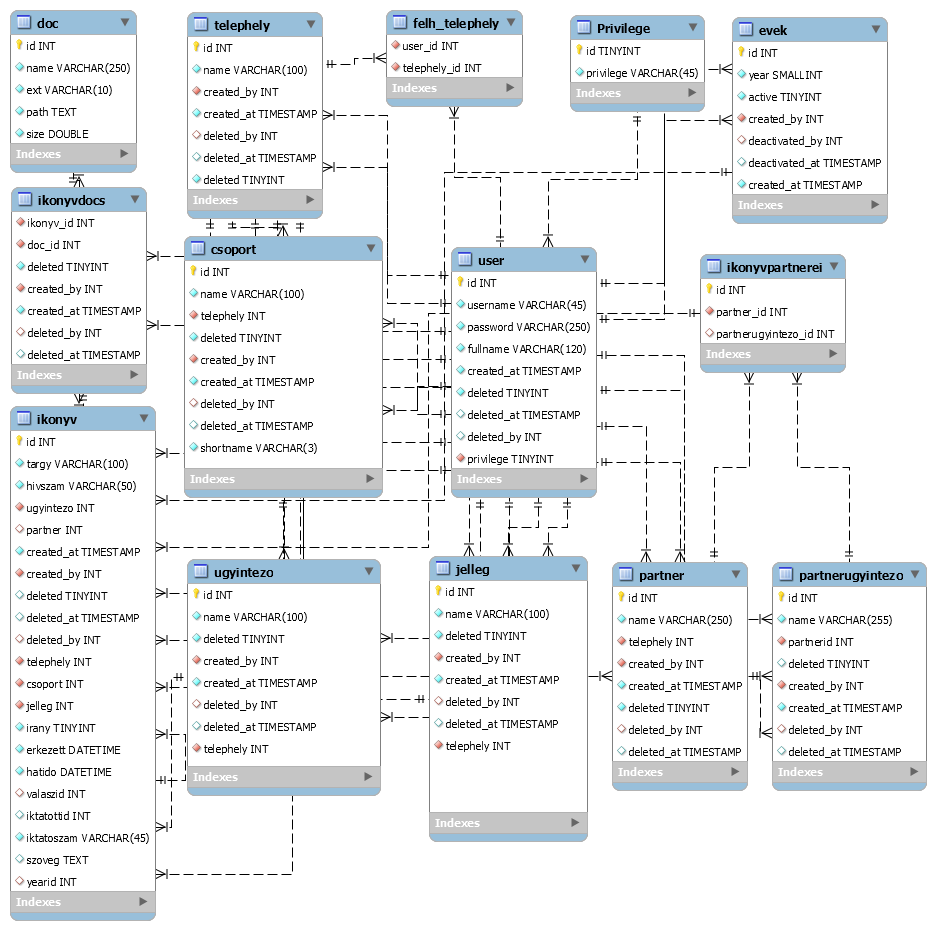
\includegraphics[width=6cm]{adatbazisterv}
	\caption{Adatbázis tervezet}
	\label{fig:adatbazisterv}
\end{figure}
Az adatbázis a következő táblákat fogja tartalmazni: Ikonyv, Ikonyvdocs, Doc, Telephely, Csoport, Ugyintezo, Jelleg, User, felh\_telephely, Privilege, evek, ikonyvpartnerei, partner, partnerugyintezo. Ahogy \az{\ref{fig:adatbazisterv}} ábrán is látható. Ezek a táblák lefedik a követelmény specifikációkban foglaltakat. Minden adatbázis művelet tárolt eljáráson keresztül végződik.

A program működésének ábrázolása use case diagram segítségével (\az{\ref{fig:usediag} } ábrán látható.)

Az egyes telephelyeken lévő felhasználók bejelentkeznek a számítógépjeiken feltelepített kliens programjuk segítségével. A szoftver egy TLS gRPC csatorna segítségével kommunikál a szerverrel.

A szerveren lévő applikációhoz a rendszergazda hozzá férhet, ahol beállításokat és mentéseket készíthet. Csak a szerver képes kommunikálni a MySQL adatbázis kezelő rendszerrel.\\
A rendszerrel szemben támasztott általános követelmények:
\begin{itemize}
	\item A rendszer funkcióit csak bejelentkezés után használhatják a felhasználók
	\item Adattárolás MySQL adatbázison
	\item A dokumentumok a szerveren kerüljenek eltárolásra időbélyegzővel a nevében
	\item A szerver és a kliens Windows platformra legyen tervezve
	\item TLS kapcsolat a szerver és a kliens között
\end{itemize}
\begin{figure}[!ht]
	\centering
	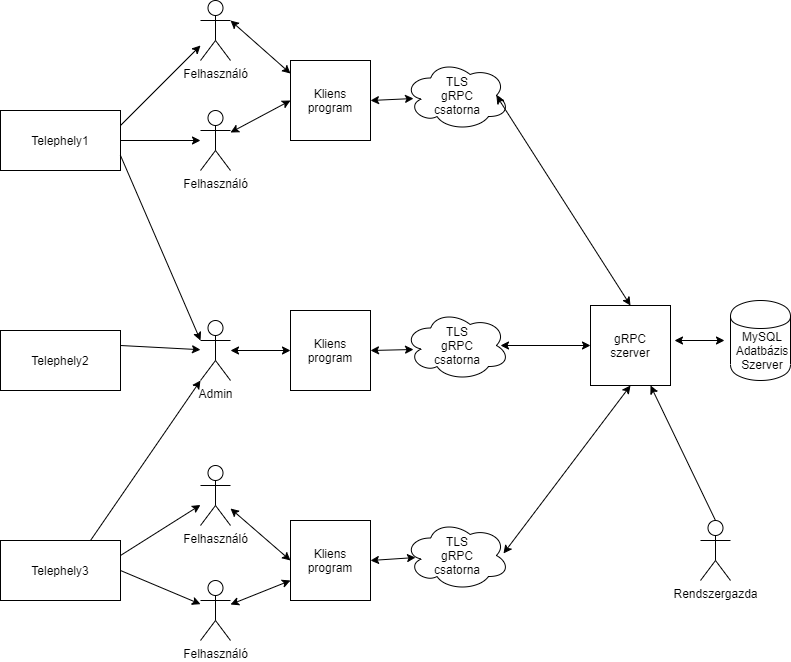
\includegraphics[width=7cm]{archdiag}
	\caption[Use Case ábra]{A szoftver működési elve.}
	\label{fig:usediag}
\end{figure}
\section{Az alkalmazással szemben támasztott funkcionális követelmény}
Felhasználókezelés
o	Admin
o	User
Törzsadatok kezelése:
Partner
Partner ügyintéző
Ügyintéző
Évek
Jelleg
Csoport
Telephely
Iktatás:
Új iktatás felvitele. A felhasználó által elkészített új iktatások megjelenítése, illetve ezekben való módosítási lehetőség.
Keresés:
Keresés paraméter alapján:
Iktatószám
Ügyintéző
Tárgy
Partner
Jelleg
Csoport
Hivatkozási szám
Szűrés év és irány alapján.
Megjelenített iktatások számának korlátozása.
Dokumentum kezelés:
Feltöltés, Megnyitás, Törlés
Adatbázis műveletek:
Mentés és helyének megadása.
Naplozási műveletek:
Naplózás helyének módosítása
Naplózási szint beállításának lehetősége
\section{Funkcionális specifikáció}
\subsection{Felhasználók számára elérhető funkciók}
\begin{enumerate}[leftmargin=0pt]
	\item \textbf{Bejelentkezés:}
	
A bejelentkezési oldalon található két szövegdoboz felhasználónév és jelszó bevitelére, valamint két gomb a bejelentkezés és kilépés. A bejelentkezés gomb a szövegdobozok adatbevitele során elérhetővé válik és be lehet jelentkezni a rendszerbe. Ha az adatok hibásak voltak arról értesíti a felhasználót. A felhasználó nevének a mentésére is van lehetőség, amit egy jelölőnégyzet bepipálásával lehet jelezni a szoftvernek. Sikeres bejelentkezés esetén a felhasználót a Főoldalra irányítjuk, ott nincs különösebb funkció csak a napi ige van megjelenítve. Kilépés gomb bezárja a programot.	
	
	\item \textbf{Törzsadatok:}
	
Az a menüpont, ahol lehetőségünk van az iktatáshoz szükséges adatok felvitelére. Alapértelmezetten az összes törzsadat letöltődik a szerverről, ezeket jelenítjük meg több lista formájában és ezek alatt jelenik meg a hozzáadás, törlés és módosítás gomb. A hozzáadás lehetőséget ad új adat felvitelére, a módosítás a kijelölt törzs javítását teszi lehetővé, a törléssel pedig eltávolíthatjuk a nem használt törzsadatot. \\Felhasználóként a következő adatok manipulációjára van jogosultságunk: 
\begin{list}{}{}
\item Ügyintéző
\item Partner
\item Partnerügyintéző
\item Jelleg
\end{list}

	\item \textbf{Iktatás:}

Az erre a célra kialakított menüpontban van lehetőség az iktatásra, ahol vannak kötelezően kitöltendő és opcionális mezők. A felhasználó csak a hozzárendelt telephelyekre iktathat.

\textit{\textbf{Kötelező mezők:}} 
\begin{itemize}
	\item Telephely: Ez egy legördülő lista, ahol a felhasználóhoz rendelt telephelyek választhatók ki.
	\item Irány: Legördülő listaelem, két választási lehetőség bejövő és kimenő.
	\item Tárgy: Ez egy szöveg beviteli mező, aminek a maximális mérete 100 karakter hosszú.
	\item Jelleg: Legördülő elem, a telephelyhez tartozó jellegeket listázza ki.
	\item Csoport: Legördülő elem, a telephelyhez tartozó csoportokat listázza ki.
	\item Partner: Legördülő elem, a telephelyhez tartozó partnereket listázza ki.
	\item Érkezett dátum: Ez egy dátumválasztó, a dokumentum beérkezési idejét vihetjük fel.
	\item Határidő dátum: Ez egy dátumválasztó, ha van a dokumentumnak határideje, akkor felvisszük, amúgy az érkezett dátumot állítjuk be neki.
\end{itemize}
\textit{\textbf{Nem kötelező mezők:}} 
\begin{itemize}
	\item Hivatkozási szám: Szöveges mező aminek a maximális mérete XXX karakter.
	\item Partnerügyintéző: Legördülő elem, a törzsből kinyert partner által meghatározott adatokat tölti be. 
	\item Megjegyzés: Ez egy szöveges mező. Az iktatáshoz egy tetszőleges hosszúságú szöveget hozzá lehet adni.
\end{itemize}
	\item \textbf{Iktatás módosítása:}
Minden felhasználó tud az iktatáson módosítani, de csak azokat az adatokat, amik magát az iktatószámot nem befolyásolják.
	\item \textbf{Dokumentum kezelés:}
	
Itt megjelennek a hozzáadott állományok, ezeket egy listában mutatjuk meg a felhasználó számára, ahol feltüntetjük a fájlok neveit, méreteit és kiterjesztésüket, illetve még itt jelenik meg a törlési lehetőség is. A lista alatt van a feltöltés, megnyitás és a mégse gomb.
\begin{list}{}{}
	\item \textit{\textbf{Feltöltés: }}Itt töltünk fel az iktatáshoz dokumentumokat, amiknek a kiterjesztése lehet pdf, docx, doc, xls, xlsx.
	\item \textit{\textbf{Megnyitás: }}Miután kijelöljük a megnyitni kívánt dokumentumot, a megnyitás gomb elérhetővé válik és rákattintás után a program letölti a szerverről és az alapértelmezett programmal megnyitja azt.
	\item \textit{\textbf{Törlés: }}Miután kijelöltük a törlésre szánt fájlt, a törlés gomb elérhetővé válik és rákkattintás után az adatbázisban a törölt változót igazra állítjuk, így az iktatáshoz feltöltött fájlok között nem fog megjelenni, viszont a szerveren elérhető marad.
	\end{list}
	\item \textbf{Keresés:}
	
Az irány és az év kiválasztása után, a szerverről letöltődnek az adatok és listában megjelenítjük őket. A keresési sávba beírt és az ott lévő legördülő listából kiválasztott keresési feltétellel szűrhetünk az adatok között. Lehetőség az adatok módosítására illetve dokumentumok kezelésére.
	\item \textbf{Kijelentkezés:}
	
A kijelentkezés gomb a menüsorban található. A felhasználót kijelentkezteti a szerverről és újra megjeleníti a bejelentkezési felületet.	
\end{enumerate}
\subsection{Adminok számára elérhető funkciók}
A felhasználók által használt funkciók ugyanúgy az adminok által is elérhetőek, csak azokat soroljuk fel, amiben a két felhasználó különbözik.
\begin{enumerate}[leftmargin=*]
	\item \textbf{Regisztrálás:}
	
	A regisztrálás a rendszergazda vagy admin által történik. Az első felhasználókat csak a rendszergazda képes létrehozni.
	\item \textbf{Iktatás törlése:}
	
Az iktatás kétszeri kattintásával a módosítások között találhatjuk meg a törlés gombot. A gomb megnyomásával töröljük az iktatást, ha az iktatás előzmény volt, akkor a hozzá csatoltak is törlődnek.	
	\item \textbf{Törzsadatok:}
	
Csoport és telephely adatok módosítására azért nincs lehetősége a felhasználónak, mert az intézményi ügyviteli szabályzat által vannak korlátozva. 	
	\begin{list}{}{}
		\item \textbf{Felhasználó:}\\
		\begin{itemize}[leftmargin=*]
			\item[] \textit{\textbf{Hozzáadása: }}A hozzáadásnál meg kell adnunk a felhasználó teljes nevét, felhasználónevét, jelszavát, jogosultsági szintjét, illetve, hogy melyik telephelyekhez tartozhat. A telephelyek kiválasztására egy legördülő menü ad segítséget, miután kiválasztottuk a telephelyet, a telephely hozzáadás gombbal tudjuk hozzárendelni a felhasználóhoz. Ezután a legördülő menüből eltűnik a kiválasztott telephely. Rontás esetén van lehetőségünk a felvitt telephely törlésére. A törölt adat visszakerül az eredeti helyére.
			\item[] \textit{\textbf{Módosítása: }}A módosítás hasonló elven működik, mint a hozzáadás. A jelszómódosításon kívül minden adatot tudunk korrigálni. A jelszómódosításra csak a rendszergazdának van lehetősége. 
			\item[] \textit{\textbf{Törlése: }}A törléssel a felhasználót inaktívvá tesszük, minden adata megmarad, csak a rendszerbe nem fog tudni bejelentkezni. Visszaállítani csak a rendszergazda tudja.
		\end{itemize}
	\item \textbf{Telephely és Csoportok:}
	Mind a két lehetőséghez lehet hozzáadni, módosítani és törölni. Ezeket igaz adminok végezhetik, de mind a két törzs adat az intézményi szabályzat mondja meg, hogy mik lehetnek. Tehát tényleges adat manipuláció nagyon nem fog történni itt. 
	\end{list}
	\item \textbf{Év zárás/nyitás:}
	
	Egy gomb ad lehetőséget az évek nyitására és zárására. Megnyomása után az aktuális évet lezárjuk és egy új évet nyitunk. Ezáltal a számozás előröl kezdődik és csak az új évre tudunk iktatni.
\end{enumerate}
\chapter{Felhasznált technológiák/eszközök}
\section{MVVM}
\subsection{MVVM bemutatása}

Az MVVM nem mást jelent, mint Model, View és ViewModel ami egy architektúrális tervezési minta. Ezt a mintát először a Smalltalk összefüggésében írták le a Xeroxnál, 1979-ben.\cite{mvvmbook} Ez a minta elválasztja a GUI (Graphical user interface)-t az üzleti logikától. Kliens oldalon szokták használni. Ebben a mintában, a modell nem jelent mást, mint az adat, amit meg fogunk jeleníteni a nézetben a nézet-modellnek a segítségével. Az MVVM-mel elő jön a tisztaság fogalma, ami a sok kódra utal a code-bihend-ban. Azaz ennek a tervezési mintának a használatával nem tárolunk kódot a xaml fájl mögött. 
\begin{figure}[ht!]
	\centering
	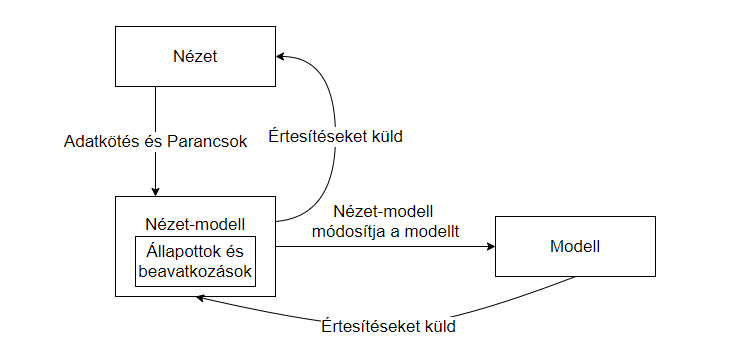
\includegraphics[height=6cm]{mvvmdiag}
	\caption[MVVM]{MVVM működése \cite{mvvmmicrosoft}}
	\label{fig:mvvmdiag}
\end{figure}
A nézet-modell úgy viselkedik, mint egy közvetítő a nézet és a modell között, és felelős a nézet logikájának a kezeléséért is. Általában, a nézet-modell interakcióba lép a modellel azáltal, hogy meghív egy eljárást a modell osztályban. Ez után a nézet-modell biztosítja az adatot a nézet számára olyan formában, hogy a nézet azt könnyedén tudja használni. A nézet-modell az adatokat a modellből szedi ki és aztán azokat elérhetővé teszi a nézet számára, előfordulhat, hogy ezeket az adatokat egyszerűbbé kell konvertálni, hogy a nézet kezelni tudja őket. A nézet-modellben találhatóak meg azok az eljárások, amik a nézetben használt XAML elemek eseményei váltanak ki. Például ha a felhasználó rá klikkel egy gombra a UI az meghív egy metódust a nézet-modellben. A nézet-modellnek még olyan feladata van, hogy a logikai állapotokat definiálja.\cite{mvvmmicrosoft}

A nézet és a nézet-modell, metódusok hívások, property-k, események, üzeneteken és adatkötésen keresztül kommunikálnak egymással. Az adatkötéshez a nézetünk adat kontextusához hozzáadjuk nézet-modellünket. Így a nézet-modell mezői, property-jei elérhetővé válnak a XAML elemeinek számára, ezáltal tudjuk megjeleníteni, frissíteni az adatokat a nézetben és befolyásolni a nézet-modell adatait. A nézet-modell nem csak a modell adatait tartalmazza és jeleníti azt meg a nézeten, hanem más propertiket is, mint állapot információ.


\subsection{MVVM keretrendszer}
\subsubsection{Caliburn Micro bemutatása}
Ez egy kicsi, de mégis erőteljes keretrendszer, amit arra terveztek, hogy megkönnyítse a programok fejlesztését minden XAML platformon. Erős MV* minta támogatottsága segít abban, hogy az applikációinkat gyorsan, kód minőség vagy tesztelhetőség feláldozása nélkül fejleszthessük. Fejlesztők: Nigel Sampson, Rob Eisenberg és Thomas Ibel. Mivel ez is egy nyílt forráskódú projekt ezért sokan mások is hozzájárultak a fejlesztéshez. A Caliburn.micro is minden sok más keretrendszer is név konvenciót alkalmaz. Ezáltal találja meg a nézet-modell a hozzá tartozó nézetet. A keretrendszernek egyetlen függősége van és az a System.Windows.Interactivity amit igazából mindenki használ amikor WPF alkalmazást fejleszt. 27.000 kód sort tartalmaz a keretrendszer.\cite{caliburn} Legfontosabb tulajdonságai: 
\begin{itemize}[leftmargin=*]
\item \textbf{Action Messages: }Az Action működése megengedi számunkra, hogy össze kössük a UI triggereit, mint például gomb nyomása a nézet-modellben található metódussal. Ez a mechanizmus lehetőséget nyújt paraméterek továbbítására is a metódusok számára. A paraméter lehet egy másik FrameworkElement értéke vagy más speciális érték, mint a DataContext vagy EventArgs. Minden paraméteren elvégez egy automatikusan típus konverziót, ami a metódus szignatúrája határozz meg. Ezek a meghívások támogatják még egy védő mechanizmus is „CanExecute”-t. Ha van a triggerelt action nevéhez hasonló metódus vagy property ami Can szóval van kiegészítve az elején akkor az blokkolhatja „disable” vagy engedélyezheti „enable” azt az elemet a UI-ban. A Caliburn.Micro ActionMassages implementációja a System.Windows.Interactivity-re épül. Ezáltal lehetőség nyílik, hogy ezt a funkciót bármilyen TriggerBase alapú triggerre használhassuk.\cite{caliburn}	
\item \textbf{Action Conventions: }A konvenciók a x:Name-re épülnek. A nézetben lévő elemet és a nézet-modellben található megegyező nevű metódusra automatikusan készít egy EventTriggert az elem által alapértelmezetten definiált eseményre, és hozzárendel egy ActionMessage-t ami metódusra fog mutatni. Ha van egy metódusunk, amit „Login”-nak hívunk és van egy gombunk UI-on aminek a neve ugyanúgy „Login” akkor arra a keretrendszer automatikusan összeköti. Így amikor a gombra rá kattintunk a login metódus fog meghívódni. Továbbá figyeli a metódus szignatúráját és a szerint építi fel az ActionMassage paramétereit. Ez csak egy lehetőség, amit bármikor kikapcsolhatunk, vagy tetszés szerint módosíthatunk. Ezeken kívül módosíthatunk, hozzáadhatunk új konvenciókat különböző elemkehez. Például, tudunk olyat is csinálni, amivel feliratkozunk a gomb MouseMove eseményére.  \cite{caliburn}
\item \textbf{Binding Conventions: }A Caliburn.Micro támogatja a konvenció-alapú adatkötést is. Ez ugyanúgy x:Name segítségével is működik. Hogyha van egy property a nézet-modellben ugyan olyan névvel, mint az elem neve akkor azt megpróbálja összekapcsolni. Mikor egy összekötés bekövetkezik akkor a keretrendszer több lépésen keresztül építi a kapcsolatot. Ezek közül mind testre szabható, mint például az adatkötés módja azaz BindingMode vagy StringFormat, ValueConverter stb\dots 	\cite{caliburn}
\item \textbf{Screen, Conductor és Collection: }A Screen, Conductor és Collection osztály felel a nézetünk életciklusáért, azaz a helyes indításért, leállításért és leállítás megszakításáért az applikációnkban. A screen-t usercontroll nézet-modellkén használják. Ezek az építő elemei a megjelenítésnek a caliburn.microban. A conductor és Collection is a Screen osztály leszármazottjai. A Conductor is lehet használni usercontrolloknál, de ezt már ablakoknál vagy oldalaknál alkalmazzák javarészt, lényege, hogy képes kezelni egy Screen típusú osztályt, amit meg tud jeleníteni. A Collectionek két fajtája van.  A Collection.AllActive és a Collection.OneActive. Mindegyik több screen befogadására képes, de az egyik egyszerre csak egy screent jelenít, meg míg a másik akár egyszerre az összeset is.
\item \textbf{Event Aggregator:  }Az aggregátor egy pub/sub tervezési mintára épülő osztály. Azaz feliratkoztatjuk az egyik osztályunkat és az üzeneteket fog nekünk küldeni attól függően, hogy a regisztrált osztály milyen IHandle<T> interfészeket implementált. Az értesítés az UI szálon történik. Támogatja a polimorfizmust is. 
\item \textbf{View Locator:  }Minden nézet-modellhez a programunkban van egy alap stratégia a hozzá tartozó nézet megtalálásához. Ezt név konvenció alapján végzi el. Például ha a nézet-modellünket elnevezzük IktatogRPCClient.ViewModels.ContainerViewMode-nek akkor a Caliburn.Micro a IktatogRPCClient.Views.ContainerView-t fogja keresni. Egy nézetnek akár több nézet-modellje is lehet. \cite{caliburn}
\item \textbf{View Model Locator: }	Attól függetlenül, hogy alapértelmezetten a Caliburn.Micro a nézet-modelltől indul ki alapértelmezetten ez módosítható. Azaz támogatja, hogy először a nézetet keresi és utána nézet-modellt ugyan azzal az eljárással, mintha ennek az ellenkezője lenne. \cite{caliburn}
\item \textbf{Window Manager: }Ez a szolgáltatás is jelzi, hogy ez a keretrendszer nézett-modell központú. Átadunk a számára egy példányt abból a nézet-modellből, amit megszeretnénk jeleníteni, ő megkeresi a hozzátartozó nézetet, beállítja az összes konvenciót, amit beállítottunk rajta és megjeleníti az ablakot. \cite{caliburn}
\item \textbf{PropertyChangedBase and BindableCollection: }	A keretrendszerben lévő implementáció lehetővé teszi számunkra, a string és lambda kifejezés alapú változás értesítéseket. Megbizonyosodik róla, hogy minden esemény ami a propertyhez kapcsolódik a UI szálon történjen. A BindableCollection az ObservableCollection leszármazottja, azaz egy egyszerű lista azonban itt is ügyel arra, hogy minden eseménye a UI szálon történjen.\cite{caliburn}
\item \textbf{Bootstrapper: }Ennek az osztálynak a segítségével tudjuk a szoftverünket elindítani és futtatni. Nem kell, mást tenni hozzá csak létrehozunk egy saját osztályt, ami a BootstrapperBase osztály leszármazottja és hozzáadjuk azt a program ResourceDictonary-be. Innen tudjuk begyűjteni még az indítási paramétereket is.\cite{caliburn}
\end{itemize}
\section{gRPC és a Protobuffer}
\subsection{gRPC bemutatása}
A gRPC rekurzív mozaik szó. A jelentése gRPC Remote Procedure Call. A google fejlesztette 2015-ben. Nyílt forráskódú. Segítségével közvetlenül meghívhatunk metódusokat egy távoli gépen, mintha az lokális objektum lenne. Könnyedén létrehozhatunk vele osztott alkalmazásokat, szolgáltatásokat. Két fő részből áll. A gRPC protokollból és a protobufferből. A többi RPC szolgáltatáshoz hasonlóan itt is előre kell definiálni a szolgáltatásokat. Ezen szolgáltatások metódusait, amelyeket a későbbiek folyamán meg lehet hívni a paraméterek megadásával. A gRPC platform független. Támogatott nyelvek: c\#, java, c/c++, Dart, Go, Kotlin, Node, Objective-C, PHP, Python, Ruby. Egyik előnye, hogy automatikusan generálja nekünk a kliens csonkokat és a szerver osztályokat.\cite{grpc}
\begin{figure}[th!]
	\centering
	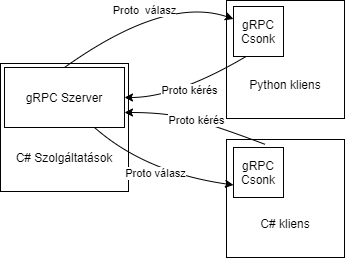
\includegraphics[width=7cm]{proto}
		\caption[gRPC]{gRPC műkődési elve \cite{grpc}}
	\label{fig:proto}
\end{figure}

\subsubsection {gRPC Protokoll}
A protokoll http2 alapokon működik és ki is használja annak előnyeit. A gRPC támogat több beépített lehetőséget, amit a http2-től örökölt. Például fejléc tömörítése, folyamatos és egyetlen TCP kapcsolat, csatlakozási, megszakítási és időtúllépési szerződések a kliens és a szerver között. A protokollnak van beépített folyamatirányítás vezérlése az adatkereteken, amit ugyanúgy a http2-től örökölt. Ez nagyon hasznos annak biztosítása érdekében, hogy az kliensek tiszteletben tartsák a rendszer teljesítményét, de extra összetettséget eredményez az infrastruktúrában felmerülő problémák diagnosztizálásakor, mivel akár az ügyfél, akár a szerver beállíthatja saját folyamatirányítási értékeit. A gRPC szerver fogja kezelni a kliens hívásokat. A kliens oldalon van egy csonk, ami azoknak a metódusoknak a fejlécét tartalmazza, amik a szerveren is megtalálhatók. Ezek segítségével fogjuk meghívni a szerver oldalon a service által definiált metódusokat. \cite{grpcprotokol}
\subsection{Protobuffer bemutatása}
A protocol buffer egy nyelvi és platform semleges protokoll, ami az adatok szerializációjáért felel. A Protocol buffer tölti be a szerződés szerepét a kliens és a szerver között. Sokkal egyszerűbb, hatékonyabb, mint egy XML struktúra és könnyebben olvasható is. Két részből áll az egyik a Message, a másik a Service, amiben az RPC-k találhatóak. 
\subsubsection{Message}
A message egy üzenet, ami az rpc híváskor adható meg paraméterként, illetve ilyen üzeneteket tud visszaküldeni a szerver. Itt lehet osztályokat kialakítani. Továbbá az rpc hívásoknál nem lehet üres a metódus, ezért létre kell hozni egy olyan Message-t is aminek nincs semmilyen mezője és ezt kell megadni paraméternek. A messagekben a skalár típusok találhatóak meg. Pl.: int32,int64,double,string,bool stb. Egy message három részből áll. Az első megmutatja az adat típusát, amit már az előbb említettek közül választhatunk ki vagy lehet egy újabb message is. A második rész a neve a mezőnek. A harmadik rész egy egyedi szám. Ez a szám segít meghatározni a mezőinket, amikor az üzenetünk bináris formátumban van.
\subsubsection{Service}
A service nem más, mint azoknak a RPC eljárásoknak gyűjtő osztálya, amit használni szeretnénk. Egy gRPC szerver több servicet is ki tud szolgálni egyszerre egy adott socketen. Alapból a compiler generál egy absztrakt osztályt és egy hozzá tartozó típus biztos csonk implementációt. A csonk fogja továbbítani a hívásokat egy gRPC csatornán keresztül.\\\textbf{A gRPC RPC típusai}
\begin{itemize}[leftmargin=0pt]
	\item[] \textit{\textbf{Unary: }}Alapvetően ezek egyszerű szinkron kérések, amiket a kliens szoftver végez a gRPC szerver felé végzünk. Egy ilyen kérés blokkolja addig a szálat amíg a szerver nem válaszol. 
	\item[] \textit{\textbf{Client streaming:  }}A szerver oldal több üzenetet fogad a kliens oldal felől, miután a kliens befejezte az adatok küldést a szerver egy válasszal zárja a kapcsolatot.
	\item[] \textit{\textbf{Server Streaming: }}Ez a kliens streamingnek a fordítottja, de itt ugyanúgy a kliens kezdi a kommunikációt. Küld egy üzenetet és erre a szerver több üzenettel válaszol. 
	\item[] \textit{\textbf{Bidirectional streaming: }}A kliens és a szerver között egy állandó kapcsolat épül ki. Egymástól függetlenül tudnak egymásnak adatokat küldeni. 
\end{itemize}
\subsubsection{Proto fájlból DLL}
Miután megírtuk a .proto fájlunkba a serviceket az rpcket és a messageket akkor van lehetőségünk őket egy protofordító segítségével olyan nyelvi kóddá fordítani, azok közül a nyelvek közül választhatunk, amiket a gRPC támogat. Ezek a fájlok tartalmazni fognak a nyelvhez illeszkedő objektumokat a messagek számára. Ezek az objektumoknak az adatait getteren és setteren keresztül fogjuk elérni. Illetve létre hoz még egy osztályt is a service-ek számára. Ha c\# nyelvet választottuk, akkor miután legeneráltattuk ezeket a fájlokat be kell tennünk a visual studioba után buildeljük és az számunkra létre hozza a DDL fájlokat. Ezeket az állományokat már könnyedén hozzáadhatjuk a szerver és a kliens oldali projektünkhöz.
\chapter{Implementálás}
\section {Kliens implementálása}
Ebben a részben be fogom mutatni a kliens oldali programom részeit. Ezeket  részeket a menü felépítésének sorrendjében fogom ismertetni. A projekt számos nézetet és nézet-modellt tartalmaz ezért csak főbb összetevőit és problémásabb részeket fogom kiemelni. A legfontosabb elemei a bejelentkezés, konténer, főoldal, iktatás, keresés, törzsek kezelése. Ezeknek a nézetekhez tartozó nézet-modellek egyes metódusait és property-jeit, és a ServerHelperSingleton osztályt fogom bemutatni röviden. A kliensre a Caliburn.Micro elérhető a nuGet package manageren keresztül amit így egy kattintással telepíthetünk. \\
\textbf{Indítás/alapbeállítás:}

Az indításhoz való legelső konfigurációs lépés nem más volt, mint az applikáció App.xml fájlja én sem tettem mást, mint a dokumentációkban leírtak alapján hozzáadtam az indító fájlt illetve kivettem a StartupUri részt az application részből.
\begin{lstlisting}[caption={App.xml},captionpos=b]
<Application.Resources>
	<ResourceDictionary>
		<ResourceDictionary.MergedDictionaries>
			<ResourceDictionary>
				<local:Bootstrapper x:Key="Bootstrapper"></local:Bootstrapper>
			</ResourceDictionary>
			<ResourceDictionary Source="style.xaml"/>
		</ResourceDictionary.MergedDictionaries>
	</ResourceDictionary>        
</Application.Resources>
\end{lstlisting}
Mint látható a ResourceDictionary-hoz egy MergedDictionary-t adtam hozzá. Az egyik dictionary tartalmazza az indítani kívánt osztályt, aminek a BootstrapperBase osztálynak az ősének kell lennie. A másik tartalmazza a szoftver formázási stílusait így XAML fájlba nem kell közvetlenül beleírnom ezeket a megjelenítési beállításokat és így azok újra felhasználhatóvá válnak és átláthatóbbá teszi a nézet kódját.
\begin{lstlisting}[caption={Indításért felelős osztály},captionpos=b]
public class Bootstrapper:BootstrapperBase
{
	public Bootstrapper()
	{
		Initialize();
	}
	protected override void OnStartup(object sender, StartupEventArgs e)
	{
		LogHelper.Initialize();
		if (e.Args.Contains("-d")) LogHelper.SetLoglevel(LogEventLevel.Debug);
		DisplayRootViewFor<LoginViewModel>();
	}
}

\end{lstlisting}
Létrehoztunk egy Bootstrapper osztályt a BootstrapperBase osztály leszármazottjaként. Az osztálynak nyílvánosnak kell lennie, hogy az App.xaml-ben is látható legyen. Felülírtuk az OnStartup metódusát annak az érdekébe, hogy a saját általunk írt Nézet-Modellt tudjuk elindítani. Ha sorról sorra megyünk a metóduson belül, akkor látszik, hogy először a LogHelper osztályt alapállapotba állítjuk. A logoláshoz a Serilog-t használom. Ha van –d paramétert indításkor akkor a logolást debug módban fogjuk beállítani így szinte mindenről fogunk tudni, hogy a felhasználó mit, mikor csinált az adott classban. Alapértelmezetten Warning-ra van állítva, azaz csak az olyan hibákat írjuk a logba ami kivételt okozott a programban. DisplayRootViewFor<T>() metódus segítségével el indítjuk a Loginunkat ahol is a T helyére beírtuk az indítani kívánt nézet-modellt. Ezután a korábbiakban leírt módon meg keresi a hozzá nézetet és megjeleníti azt.\\
\textbf{Bejelentkezés:}

Ebben a nézet-modellben összesen három property található. Ezekbe tárolom el a felhasználó adatait, illetve, egy bool propertyt, ami jelzi, hogy a felhasználó szeretné-e, hogy elmentsük a jelszavát. Ha szeretné a jelölő kattintásával módosítja a nézet-modellben található property-t és bejelentkezéskor az adatot a windows registrybe mentem. Ennek a segítségére megtalálható három konstans, ami az adat elérési útját tartalmazza. Ezen kívül megtalálható egy privát mező is, ami a UserHelperSingleton osztály, mivel a Login lehetőség ebben az osztályban érhető el. Több metódus is a rendelkezésünkre áll ezek közül a legfontosabb a szerverhez való csatlakozásra használt.

\begin{lstlisting}[caption={Bejelentkezés},captionpos=b]
async Task<bool> ConnectToServerAndLogin()
{
	CheckUsername();
	CheckPassword();
	Log.Debug("{Class} Csatlakozas a szerverhez", GetType());
	bool success = await userHelper.Login(GetDataFromLoginTextBoxes());
	if(success)Log.Debug("{Class} Sikeres csatlakozas", GetType());
	else Log.Debug("{Class} Sikertelen csatlakozas", GetType());
	if (SaveUsernameIsChecked) Registry.SetValue(keyName, "Felhasznalonev", UsernameBox);
	else Registry.SetValue(keyName, "Felhasznalonev", "");
	return success;
}
\end{lstlisting}
Ez egy async metódus annak érdekében, hogy ne blokkoljuk a UI threadet a csatlakozás közben így a kis töltést jelző indikátorunk nyugodtan futhat rajta. Az elején ellenőrizzük a felhasználó által beírt adatokat, ha hiba van az adat kitöltésben például nem írt be jelszót vagy túl rövid alapból, akkor egy InvalidUserNameExceptiont dobunk és ezzel megszakítjuk a metódus működését. Ha minden rendben van, elküldjük a beírt adatokat a szerver felé. Sikeres bejelentkezéskor megnyitjuk a konténer nézetet és abban egyből a főoldalt, illetve el tároljuk a válaszban kapott tokent. Hibás jelszó esetén a gRPC szerver kivált egy kivételt, amit eljuttat a kliens oldalra és ott jelezzük a felhasználónak azt.\\
\textbf{Konténer:}

Ebben a nézetben található meg a menüsor, illetve itt fog változni az egész program. Azaz amikor egy menü gombra rákattintunk, ami nem kilépés vagy kijelentkezés akkor az adott usercontroller betöltésre kerül. Ez egy conductor osztály amit a caliburn.micro keretrendszere nyújt. Így mindig lehet egy aktív screenem. Ennek a segítségére létre hoztam egy külön osztályt, amit SceneManager-nek neveztem el. Ennek az osztálynak van egy CreateScene függvénye, aminek egy paramétere a Scenes enumok közül választható. Visszatérési érteke egy screen osztály béli objektum. A Scenes enumok nem mást tartalmaznak, mint a megjeleníthető nézetek listáját. 

\begin{lstlisting}[showstringspaces=false,caption={Nézet váltás metódusa},captionpos=b]
private void ChangeScene(Scenes scene) {
	Log.Debug("{Class} Oldal valtasa {Scene}", GetType(),scene);
	ActivateItem(SceneManager.CreateScene(scene));
}
\end{lstlisting}
Ezt a metódust a gombokhoz hozzárendelt metódusok hívják meg. Így egy helyen történik a „jelenet” váltás. Az ActivateItem a Conductor osztály egy metódusa, aminek a bemenő paramétere egy Screen objektum. Ez a metódus fogja a nézetben található contentcontrol elembe beletenni a meghívott usercontrollt. Ezt is név konvenció alapján köti össze a telepített keretrendszer. A contentcontrollnak „ActiveItem”-nek kell lennie az x:Name mezőjében.\\
\textbf{Főoldal:}

A főoldalon egy üdvözlő üzenet jelenik meg, illetve a vágyálom rendszerben is megfogalmazott napi ige. Erre a főoldal nézet-modellje az ige modellt használja. Az ige osztály három propertyből áll és két mezőből. A LetoltottIgeDatuma jelzi, hogy mikor volt letöltve az ige. Ennek van egy alapértelmezett dátuma, ami biztos kisebb, mint az aktuális nap dátuma. Van egy property aminek csak getterje van, ez a property szolgáltatja a címet, ami magába foglalja az aktuális nap dátumát. Az utolsó pedig maga a napi ige tárolására szolgál. A főoldalon ezt a modellt statikusként állítottam be, annak érdekében, hogy a nézet-modell ne végezze el az ige adatok letöltését és formázást, csak ha szükséges. A letöltéshez a következő metódust használom:
\begin{lstlisting}[caption={Ige letöltése és formázása.},captionpos=b]
private async void DownloadIge()
{
	try
	{
		string result = "";
		using (WebClient client = new WebClient())
		{
			client.Encoding = Encoding.UTF8;
			result = await client.DownloadStringTaskAsync("https://napiige.lutheran.hu/igek.php");
		}
		_ige.NapiIge = BuildDailyIge(result);
		_ige.LetoltottIgeDatuma = DateTime.Today.Date;
		NotifyOfPropertyChange(()=>NapiIge);
	}
	catch (WebException e)
	{
		InformationBox.ShowError(e);
	}
}
\end{lstlisting}
Az aszinkronitás itt is megvan  azért, hogy a UI szálat ne foglaljuk le. Először létrehozok egy WebClient ami a System.Net névtérből származik. A kliensnek beállítom a kódolását. Ezután a fenntartótól kapott API –n keresztül leszedem a napi igét. Ezek után formázom azt reguláris kifejezések segítségével és egy kis trimmeléssel mivel ezek forráskódként kerülnek letöltésre, majd beállítom a letöltésnek a dátumát és szólok a UI-nak, hogy frissítse a NapiIge-vel összekötött elemét. Hiba esetén jelzem azt a felhasználó számára.\\
\textbf{Iktatás:}

Az iktatás nézetében, megtalálható az összes kötelező törzs adat kiválasztási lehetősége. Ezeket legördülő menü formájában találja meg a felhasználó a felületen. Ezek mindegyikéhez a nézet-modellben tartozik egy név azonos property, illetve a kijelölt elemek számára is. A nézet-modell-t az IkonyvHandlerből származtatom, ami tartalmazz két IHandle interfészt és a Screen osztály leszármazottja. Ezt a segéd osztályt azért hoztam létre, hogy csoportosítsam egy helyre azokat a tulajdonságokat egy nézetnek, amit muszáj kezelnie, ha tartalmaz olyan DataGridet amiben iktatásokat jelenít meg. Három metódus tartalmaz ebből kettő absztrakt, hogy azt a gyermekosztály majd megvalósítsa. Az iktatókönyv módosítására való metódus viszont mindenhol ugyan az, ezért azt már itt implementáltam. 
\begin{lstlisting}[caption={Iktatás módosítása ablak megnyítása WindowManager segítségével.},captionpos=b]
public void ModifyIkonyv() {
	if (SelectedIkonyv == null) return;
	WindowManager windowManager = new WindowManager();
	Screen screen = new PopUpViewModel(new ModifyIkonyvViewModel(_selectedIkonyv));
	windowManager.ShowDialog(screen);	
}
\end{lstlisting}
Ebben a metódusban található egy WindowManager, ami az új ablak megnyitásáért felelős a Caliburn.Micro keretrendszerben. A ShowDialog függvénynek a bemeneti paramétere egy PopUpViewModel lesz, aminek át adunk egy másik nézet-modellt ez pedig az iktatás módosítására használt objektum. A PopUp nézetett azért hoztam létre, hogy az ablak mögötti rész el sötétítése egy helyen történjen, ne kelljen folyamatosan újra implementálnom, a hibákon kívül minden felugró ablak ezen a nézet-modellen keresztül fog megjelenni. 

Az iktatás nézet-modell konstruktorában először csak a telephelyeket szedem, le az adatbázisból majd beállítom az első lehetséges telephelyet. Ennek hatására megindul a telephelyhez tartozó adatoknak is a letöltése. 
\begin{lstlisting}[showstringspaces=false,caption={Iktatáshoz szükséges adatok letöltése.},captionpos=b]
private async void LoadData()
{
	Log.Debug("{Class} Adatok betoltese a szerverrol.", GetType());
	SelectedIrany = Iranyok.First();
	eventAggregator.Subscribe(this);
	AvailableTelephelyek = await serverHelper.GetTelephelyekAsync();
	if (AvailableTelephelyek.Count > 0) SelectedTelephely = AvailableTelephelyek.First();
	Log.Debug("{Class} Sikeres adat letoltes.", GetType());
}
\end{lstlisting}
Az irányok belevannak „égetve” az osztályba, mert ezek nem fognak változni. Alapértelmezetten kijelöli a „bejövő” részt, tehát erre fog iktatni a felhasználó, ha ezt nem módosítja. A konstruktorban még fel is iratkozok a Caliburn.Micro által nyújtott EventAggregatorra. Az eventAggregator segít abban, hogy az osztály értesítéseket kapjon azokról az eseményekről, amikre az IHandle interfészek által feliratkozott Az IHandle implementálni kell, mivel a KonyvHandler osztályban nincsenek.\\
A Handlerek implementációja:
\begin{lstlisting}[caption={Iktatás törlése a táblából.},captionpos=b]
public override void Handle(RemovedItem message)
{
	if (message.Item is Ikonyv)
	{
		_recentlyAddedIkonyvek.Remove(message.Item as Ikonyv);
		NotifyOfPropertyChange(() => RecentlyAddedIkonyvek);
	}
}
\end{lstlisting}
A RemovedItem handler arra szolgál, ha törölné a felhasználó az éppen felöltött iktatást, akkor az a statikus Iktatókönyvek közül kitörölje. 
\begin{lstlisting}[caption={Iktatás módosítása a táblában.},captionpos=b]
public override void Handle(Ikonyv message)
{
	for (int i = 0; i < RecentlyAddedIkonyvek.Count; i++)
	{
		if (RecentlyAddedIkonyvek[i].Id == message.Id)
		{
		RecentlyAddedIkonyvek.RemoveAt(i);
		RecentlyAddedIkonyvek.Add(message);
		}
	}
}

\end{lstlisting}
A módosított iktatásokat kapja el. Ha egy módosítás bekövetkezik, akkor azt kitöröli a nem rég hozzáadott iktatókönyvek közül és hozzáadja az új módosított objektumot.

Ha a felhasználó iktatni szeretne és elkezdi ki tölteni a mezőket, azt folyamatosan ellenőrizzük, ha a bevitt adat elegendő és az összes kötelező mezőt kitöltötte, akkor az iktatási gomb, ami alapértelmezetten kikapcsolt állapotba van, bekapcsoltra állítjuk. Ennek a funkciónak a megkönnyítésére is van lehetőség Caliburn.Micro-ban amit ugyanúgy névkonvenció alapján összetudja kötni a logikai propertyt a XAML elemmel. A gombot el neveztük IktatButton-nak, így a publikus property, amit létre kell hoznunk az a CanIktatButton.
Ezen a property-n belül csak vissza adom az én saját private logikai függvényem értékét ahol történik az igazi ellenőrzés. 
\begin{lstlisting}[caption={Iktatáshoz tartozó adatok validálása.},captionpos=b]
private bool FormValidation() {
	bool IsValid = true;
	if (IsTorzsDataInFormNull()) IsValid = false;
	else if (string.IsNullOrWhiteSpace(Targy)) IsValid = false;
	else if (Targy.Length > 100) IsValid = false;
	else if (DateTime.Parse(HatidoDatum) < DateTime.Parse(ErkezettDatum)) IsValid = false;
	else if (ValaszIsChecked && SelectedIktSzam == null) IsValid = false;
	else if (Szoveg.Length > 500) IsValid = false;
	else if (Hivatkozasiszam.Length > 50) IsValid = false;
	return IsValid;
}
\end{lstlisting}
A függvény folyamán ellenőrzöm a szöveges mezők számának a hosszát, hogy az nem haladta-e meg az adatbázisban foglalt oszlop maximális karakter számát. Továbbá ellenőrzöm még azt, hogy a határidő dátuma ne legyen kisebb, mint az érkeztetés dátuma és még azt is, hogy minden kötelező mező ki lett-e töltve. Ha ez sikeres, akkor az iktatás gombra rá tudunk kattintani, ahol nem történik más, mint létrehoz egy új iktatási objektumot, amit átadunk a ServerHelperSingleton által szolgáltatott AddIktatas függvénynek. 

A függvény bemeneti paramétere egy Ikonyv típusú objektum a kimeneti paramétere egy RovidIkonyv, ami csak az Id-t és az iktatószámot fogja tartalmazni. Ez a gRPC által generált kliens csonkot fogja használni arra, hogy a szerverre elmentse az adatokat. 
\begin{lstlisting}[caption={Iktatás hozzzáadása.},captionpos=b]
public async Task<RovidIkonyv> AddIktatas(Ikonyv newIkonyv)
{
	RovidIkonyv rovidIkonyv = new RovidIkonyv() { Id = 0 };
	try{
		rovidIkonyv = await Client().AddIktatasAsync(newIkonyv, GetCallOption());
	}
	catch (RpcException ex)	{
		InformationBox.ShowError(ex);
	}
	catch (Exception e){
		InformationBox.ShowError(e);
	}
	return rovidIkonyv;
}

\end{lstlisting}
A visszatérés után megjelenítjük a felhasználónak az új iktatószámot és a kiegészített adatokkal hozzáadjuk a RecentlyAddedIkonyvek propertyhez. Ezáltal meg fog jelenni a nézetben is.\\
\textbf{Keresés:}

A keresés is gyermek osztálya a IkonyvHandler osztálynak. Első lépésként leszedem a szerverről az elérhető éveket és beállítom a lehetséges irányokat. Amint a felhasználó mind a két legördülő menüből kiválasztott egy lehetőséget megkezdődik a szerverről az iktatásoknak a letöltése. Az adatok megjelenítéséhez három BindableCollection<Ikonyv> property-t kell, amik a következők: AllIkonyv, SearchedIkonyvek, ShownIkonyvek. Az első property tartalmazza az összes iktatást, amit leszedtünk, a második tartalmazza azokat az adatok, amik megfelelnek a keresési kritériumoknak és a harmadik maga a megjelenített iktatások. A megjelenítéskor figyelembe veszem, hogy a felhasználó hány darab iktatást szeretne megjeleníteni az oldalon és csak annyit jelenítek meg. Az oldalak kezeléséhez a gombokat le kell generálni, aminek darabszámát mindig a SearchedIkonyvek található adatok száma és a megjeleníteni kívánt iktatás oldalanként határozza meg. Az összes letöltött adat darab számát megjelenítem.
\begin{lstlisting}[caption={Megjeleníthető iktatások a keresésben.},captionpos=b]
private async void SetVisibleIktatas() {	
	if (AllIkonyv.Count == 0) return;
	await SetSearchData();
	ShownIkonyvek.Clear();
	if ((CurrentPage+1) * SelectedItemsPerPage > SearchedIkonyvek.Count)
	{
		for (int i = (CurrentPage ) * SelectedItemsPerPage; i < SearchedIkonyvek.Count; i++)
		{
			ShownIkonyvek.Add(SearchedIkonyvek[i]);
		}
	}
	else 
	{
		for (int i = CurrentPage * SelectedItemsPerPage; i < CurrentPage * SelectedItemsPerPage + SelectedItemsPerPage; i++)
		{
			ShownIkonyvek.Add(SearchedIkonyvek[i]);
		}
	}
	NotifyOfPropertyChange(() => ShownIkonyvek);	
	SetButtons();
	NotifyOfPropertyChange(() => MaxItemNumber);
} 
\end{lstlisting}

A megjelenítésnek a folyamata a következő képen zajlik. Ellenőrzöm, hogy van-e egyáltalán iktatás a listánkban, ha nincs kilépek az eljárásból. Utána megnézem, hogy a felhasználó beírt-e valami keresési feltételt, ha igen akkor annak alapján beállítom a SearchedIkonyv propertyt miután ez megtörtént megnézem, hogy kitudom-e íratni az összes talált iktatást, ha nem akkor megnézem, hogy melyik oldalon is vagyunk és az alapján iratom ki azokat. Miután ezt befejeztem szólok a nézetnek, hogy frissítse a kötéseket, beállítom a gombokat és jelzem a talált iktatások számát.\\
\textbf{Törzs:}

A nézet-modell a Collection.AllActive gyermek osztálya. Mint azt már korábban említettem, ez az osztály abban különbözik a Conductor osztálytól, hogy több Screen eleme is lehet és egyszerre ezek közül többet is meg tud jeleníteni. Ahhoz hogy megjelenítsük ezeket a nézet-modelleket nincs más teendőnk, mint létrehozni minden egyes megjeleníteni kívánt Screen típusú osztálynak egy property-t amit a caliburn.micro össze köt a XAML-ben található contentcontroller elemekkel. Itt megnézzük, hogy a felhasználó admin-e ha igen, akkor az összes beállítási lehetőségeket megkapja. Ebben a törzs nézet-modellben történik még meg a telephelyek letöltése és publikálása, de csak miután megjelenítettük és felírattuk az összes többi nézet-modellt az eventaggregatorra. 
\begin{lstlisting}[showstringspaces=false,caption={Telephelyek letöltése a törzs adatok számára.},captionpos=b]
private async void GetTelephelyekAsync() {
	Log.Debug("{Class} Telephelyek letoltese.", GetType());
	LoaderIsVisible = true;
	BindableCollection<Telephely> telephelyek = await 	ServerHelperSingleton.GetInstance().GetTelephelyekAsync();
	await eventAggregator.PublishOnUIThreadAsync(telephelyek);
	LoaderIsVisible = false;
}
\end{lstlisting}

Mint látható a TorzsViewModel is a ServerHelperSinglton osztályt alkalmazza az adatok letöltésére. Miután ez megtörtént az EventAggregatornak van egy metódusa, hogy PublishOnUIThreadAsync(), aminek a bemeneti paraméter egy object osztály. Tehát bármilyen osztályt alkalmazhatunk ezáltal. Ezután a hívás után azok az elemek is elkezdhetik a saját adataiknak a letöltését a szerverről, amelyek implementálták az IHandle<Telephely> interfészt. Mindegyik nézet-modell implementálja azokat az IHandle<T> interfészeket, amikre szükségük van. Ebben a menüpontban van a legjobban kihasználva az EventAggregator és az ServerHelperSingleton osztálynak a tulajdonságai.  Mindegyik törzset kezelő felület tartalmazza a szerver elérésére létrehozott egyke osztályt, ennek hála mindegyik lekérdezés ugyan azon a csatornán fog végződni mivel ebből az osztályból csak egy van az egész program futtatása alatt. \\

\textbf{Dokumentumkezelés:}

A dokumentum kezelésre minden olyan felületnek van lehetőség amelyik implementálja a IkonyvHandler osztályt. Ugyanis az iktatáshoz tartozó dokumentumok kezelésére a módosítás közben van lehetőségünk. Amint rákattintunk kétszer egy iktatásra a DataGrid-en, az egy új ablakot fog megjeleníteni ahol is található a dokumentumok gomb. Ennek a gombnak a megnyomására jelenik meg az a felület, ahol látjuk az összes dokumentumot és ahol fel is tudunk tölteni újat. A dokumentum megnyitása úgy történik, hogy kijelöljük a megnyitni kívántat és rákattintunk a megnyitás gombra. Ennek hatására a DownloadDocument metódus fog meghívódni.
\begin{lstlisting}[showstringspaces=false,caption={Dokumentum letöltése.},captionpos=b]
public async void DownloadDocument() {
	try
{
LoaderIsVisible = true;
	Document rawdata = await serverHelper.GetDocumentByIdAsync(SelectedDocument);
	if (rawdata.Id != -1){
		byte[] bytes = rawdata.Doc.ToByteArray();
		string temppath = Path.GetTempPath();
		string fullpath = $"{temppath}{rawdata.Name}.{rawdata.Type}";
		if (File.Exists(fullpath)){
			File.Delete(fullpath);
			File.WriteAllBytes(fullpath, bytes);
		}
		else File.WriteAllBytes(fullpath, bytes);
		Log.Debug("{Class} Sikeres adatmentes.", GetType(), SelectedDocument);
		try{
			Process.Start(fullpath);
		}
		catch (Exception e){
			InformationBox.ShowError(e);
		}
	}
	else{
		MessageBox.Show("Hiba a dokumentum letoltese kozben.");
	}
	LoaderIsVisible = false;
	catch (Exception e){
		InformationBox.ShowError(e);
	}
}
\end{lstlisting}

A függvény először vár az adat letöltésére, ha sikerült, akkor visszakapjuk annak a fontos információit és magát a dokumentumot. Ha az Id mező nem egyenlő -1 -el akkor megyünk tovább. Az adatokat berakjuk byte tömbbe, lekérjük a rendszertől az ideiglenes fájlok tárolására használta mappának az elérési útvonalát. Ha ez sikeres, akkor konkatenáljuk ezt az útvonalat a letöltött dokumentum nevével. Ha már letöltötték ezt a fájlt, akkor először kitöröljük, majd újra kiírjuk a lemezre, ha nem akkor csak kiírjuk. Ezután a Process.Start() segítségével megnyitjuk az állományunkat. Ennek a metódusnak több változata is van, de én a string paramétereset hívom meg, ami fájl vagy dokumentum elérési útvonalának kell lenni ennek hatására elindítja az alapértelmezett programmal azt.

A feltöltés gomb az UploadDocument metódust indítja el. Először megjelenítjük a c\# által támogatott fájl kiválasztót, ha ott sikeresen kijelöltünk egy fájlt létrehozunk egy új Document objektumot. Itt minden információt megadunk a fájlról és beolvassuk a Doc mezőjébe a fájl adatait.
\begin{lstlisting}[showstringspaces=false,caption={Dokumentum feltöltése.},captionpos=b]
public async Task UploadDocument() {

	string[] FileInfo = ChooseDataToUpload();
	if (string.IsNullOrWhiteSpace(FileInfo[2])) return;
	LoaderIsVisible = true;
	Document document = new Document();
	document.Name = FileInfo[0];
	document.Type = FileInfo[1];
	document.Doc = ByteString.CopyFrom(GetBytesFromFile(FileInfo[2]));
	document.IkonyvId = ikonyvid;
	DocumentInfo uploadedDocument = await serverHelper.UploadDocumentAsync(document);
	if (uploadedDocument.Id != -1)
	{
		Log.Debug("{Class} Sikeres feltoltese. ", GetType());
		IkonyvDocuments.Add(uploadedDocument);
		NotifyOfPropertyChange(() => IkonyvDocuments);
		ModificationHappend = true;
	}
	else {
		Log.Debug("{Class} Sikertelen feltoltese. ", GetType());
		MessageBox.Show("Sikertelen feltoltes.");
	}
	LoaderIsVisible = false;
}
\end{lstlisting}
Sikeres beolvasás után elindítjuk a feltöltést, ellenőrizzük annak sikerességét. Hozzáadjuk a dokumentumot a jelenlegiekhez és értesítem a nézetet a változásokról.\\
\textbf{SeverHelperSingleton:}

Ez az osztály a legfontosabb a szerver eléréséhez, ugyanis ő használja a kliens csonkokat. Ő az egyke osztályok azon fajtáját reprezentálja, amit úgy hívunk, hogy „mohó”. A mohó osztály annyiban különbözik a „lustától” hogy alapból szálbiztos, de erőforrásait egyből inicializálja. A csonkok használatán kívül más feladatai is vannak. Az egyik a gRPC csatorna létrehozása és annak lezárása a másik, hogy a hitelesítési adatokat mindig elküldje a http2 fejlécében a szerver számára.
\begin{lstlisting}[showstringspaces=false,caption={gRPC csatorna készítése.},captionpos=b]
private void CreateNewChannel() {
	string hostname = ConfigurationManager.AppSettings["Hostname"];
	string hostport = ConfigurationManager.AppSettings["Port"];
	string csatinfo = $"{hostname}:{hostport}";
	var servercert = File.ReadAllText("cert/server.crt");
	SslCredentials creds = new SslCredentials(servercert);
	channel = new Channel(csatinfo, creds, new[] {
		new ChannelOption("grpc.keepalive_permit_without_calls", 1),
		new ChannelOption("grpc.http2.max_pings_without_data",0),
		new ChannelOption("grpc.keepalive_timeout_ms",50),
		new ChannelOption("grpc.keepalive_time_ms",360000)
	});
}
\end{lstlisting}
A csatorna létrehozása során beolvassuk az app.config fájlban található csatlakozási adatokat. Ezeket az adatokat egy socketté állítjuk össze. Ezután beolvassuk a hitelesítést, amit a gRPC névtérben található SslCredentials objektum létrehozásához használunk. Ha ez megtörtént létrehozzuk magát a csatornát. A csatorna bemeneti paraméterei a socket, hitelesítés, és az általunk konfigurált csatorna beállítások. Ezeknek a beállításoknak meg kell egyeznie a szerveren lévővel, különben a szerver bonthatja a kapcsolatot hibás konfigurációra hivatkozva. Ezek az opciók arra szolgálnak, hogy a kapcsolat ne szűnjön meg, hogyha a program egésznap is fut, és nem történik egy gRPC hívás sem.

A fejlécbe történő adat beágyazás nem bonyolult. Ugyanis a gRPC-nél minden híváshoz megadhatók hívási beállítások. Ezek között a találjuk meg a http2 protokoll fejlécét is.
\begin{lstlisting}[showstringspaces=false,caption={CallOption beállítása.},captionpos=b]
private CallOptions GetCallOption() {
	return new CallOptions().WithHeaders(new Metadata(){
			new Metadata.Entry("Authorization", userHelper.Token.Token)
		});
}
\end{lstlisting}
Ezért úgy oldottam meg, hogy minden egyes híváshoz lekérünk új CallOptions –t amibe beleágyazom a tokent, amit a bejelentkezéskor kapott meg a felhasználó. 
\section {Szerver implementálása}
A szervernek is egy kisebb WPF applikációt hoztam létre, itt nem használtam már semmilyen keretrendszert. A szerverben implementáltam a gRPC protobuffer által generált szolgáltatásokat, MySQL adatbázisban található adatok manipulálásához a szükséges osztályokat, illetve a rendszergazdai kezelő felületet.  A kezelő felületek között megtalálható a naplózás beállításainak lehetősége, adatbázis mentése és a felhasználók létrehozása illetve módosítása jelszóval együtt.\\
\textbf{Adatbázis kezelő osztályok:}

Minden adatbázis kezelő osztályomnak két kötelező interfészt kell implementálnia. Az egyik IDatabaseConnectionManager<T>, a másik pedig a 11 IManage(adat) interészek közül az egyik, ami ugye attól függ, hogy melyik adatnak a manipulációjával fog foglalkozni.

A csatlakozásért felelős interfészt, két metódust, egy függvényt és egy propertyt tartalmaz.
Ez egy generikus interfész, így bármelyik adatbázis kezelőnek a csatlakozást megadhatjuk neki (Pl.: MySqlConnection).
\begin{lstlisting}[caption={Kötelező interfész adatbázist kezelő osztályok számára.},captionpos=b]
public interface IDatabaseConnectionManager<T>
{     
	ConnectionManager ConnectionManager { get;  }
	void OpenConnection(T connection);
	void CloseConnection(T connection);
	T GetConnection();
}
\end{lstlisting}
A property nem más, mint egy ConnectionManager osztály, ami annyit csinál, hogy kiszedi az applikációnk konfigurációs fájljából a szükséges adatbázis információkat. Az OpenConnection és a CloseConnection fog felelni az adatbázis kapcsolat helyes nyitásáért és bezárásért. A bemeneti paraméterek a T osztály. Visszatérési értéke nincs, mivel ha hiba történik valamelyik metódus közben, akkor kivételt váltunk ki, amit elkapunk és beleírjuk a naplófájlba. A GetConnection pedig visszaadja a kapcsolatot az adatbázis műveletet végző osztályaink számára.

A másik interfészre egy példa a IManagePartner. Ő sem tartalmazz mást csak azokat a függvényeket, amik szükséges a Partner adatainak a manipulációjához. Interfészek használatával megfelek a GOF1-ben foglaltaknak azaz később a Service osztályomba ezekre fogok tudni hivatkozni.\\
\begin{lstlisting}[caption={Kötelező interfész partnereket kezelő osztályok.},captionpos=b]
interface IManagePartner
{
	Partner AddPartner(NewTorzsData newObject, User user);
	Answer DeletePartner(int id, User user);
	List<Partner> GetPartnerek(Telephely filter);
	Answer ModifyPartner(Partner modifiedObject);
}
\end{lstlisting}
Ebben az interfészben megtalálható az AddPartner függvény, aminek a bemeneti paramétere egy protobuffer fájlban meghatározott message, ami a NewTorzsData, ez az osztály tartalmazza a törzs adatokat, így bármelyik belehelyezhető. Illetve bekér még egy felhasználót is, erre azért van szükség, mert az adatbázisba csak így tudjuk eltárolni, hogy éppen ki mit csinált. Visszatérési érteke egy Partner típusú objektum. A DeletePartner bemeneti érteke egy partnernek az id-je, illetve ugyanúgy bekérem a usert is hasonló szándékok miatt. Visszatérési értéke egy Answer message, ami tartalmaz egy string, és egy bool propertyt. Ezeket arra használom, hogy a kliens felé tudom jelezni, ha valami hiba történt és egyből a szervertől fogja megkapni a hiba pontos leírását is. \cite{errorhandling}Letudom kérni a telephelyenkénti partnereket is a GetPartnerek segítségével, így a bemeneti paraméter egy Telephely osztály lesz a kimenete pedig partnerek listája. Az utolsó függvény a ModifyPartner, aminek a bemeneti értéke a módosított partner, ez mindent tartalmaz ami számunkra fontos az adatbázisban való módosításhoz. Visszatérési értéke ugyanúgy egy Answer, mint a törlésnél.

Az ismétlés elkerülése végett az IDatabaseConnectionManagert egy absztrakt osztályba implementáltam, de már megadtam a generikus változójának az értéket. Ennek az osztálynak a neve MysqlDatabaseManager. Ez egy kis osztály, de annál fontosabb, így minden MySql-el foglalkozó osztálynak csatlakozásáért itt tudom befolyásolni. Illetve ha pontosabb hiba kezelést akarok az adatbázis kapcsolat zárása vagy nyitásához, akkor csak itt fog kelleni módosítani.

Minden IManage(adat) interfészhez létrehoztam egy service osztályt is. Ezek a service osztályok fognak megjelenni a gRPC szolgáltatásai között, így ha le akarom cserélni az adatbázis osztályt vagy egy másik adatbázis kezelőt kell implementálnom nagyban megfogja könnyíteni a dolgomat, mert ez az osztály dependency injectiont és dependency delegationt használ. 
\begin{lstlisting}[caption={A partnerekkel foglalkozó osztály.},captionpos=b]
class PartnerService:IManagePartner
{
	IManagePartner dbManager;
	public PartnerService(IManagePartner dbManager)	{
		this.dbManager = dbManager;
	}
	public Partner AddPartner(NewTorzsData newObject, User user){
		return dbManager.AddPartner(newObject, user);
	}
	public Answer DeletePartner(int id, User user){
	return dbManager.DeletePartner(id, user);
	}
	public List<Partner> GetPartnerek(Telephely filter){
		return dbManager.GetPartnerek(filter);
	}
	public Answer ModifyPartner(Partner modifiedObject){
		return dbManager.ModifyPartner(modifiedObject);
	}
}

\end{lstlisting}
Az osztálynak van egy IManagPartner mezője ezt a mezőt a konstruktorába paraméterként várom. Ebben az osztályban minden metódus a dbManager-re támaszkodik. Ez igazából csak egy közvetítő osztály. Viszont ennek hatására a programom könnyebben tesztelhetővé vált. Ezeknek az osztályoknak már egy teljesen implementált adatbázis kezelő osztályt fogok átadni.

PartnerDatabaseManager ebben az osztályban már az összes metódus az adatbázis műveletekkel foglalkozik, mivel örökölte a MysqlDatabaseManagertől a kapcsolódási metódusokat. Ezeket fogom átadni inicializáláskor a servicek számára.\\
\textbf{Adatbázis kezelő osztályok:}

Ez az osztály implementálja az összes olyan szolgáltatást amit a gRPC szervernek tudnia kell. A szolgáltatás osztályunknak az ősosztálya az IktatoService.IktatoServiceBase. Ebben az ősosztályban minden metódus virtuális így az általunk készített osztályban felülírhatjuk őket a saját logikánkkal. A ServiceForgRPC osztály összesen 48 eljárást tartalmaz. Ebből 46 gRPC hívásokkal foglalkozik, míg a maradék kettő közül az egyik a felöltött fájlok beolvasásáért felel, a másik ellenőrzi, hogy a hívásokból érkező fejlécekben érvényes-e a felhasználói adat. A gRPC hívások nagyon egyszerűek, nekem így már csak annyi volt a feladatom, hogy meghívtam a MySQLDatabaseManager által szolgálatot valamelyik függvényét és annak a visszatérési értékét csak vissza kell küldenem válaszként. Minden gRPC hívásból bemutatok egyet, kivéve a kétirányú távoli eljárást.
\begin{itemize}[leftmargin=0pt]
	\item \textbf{ServerStreaming: }
	\begin{lstlisting}[showstringspaces=false,caption={Iktatások küldése a kliens számára.},captionpos=b]
public override async Task ListIktatas(SearchIkonyvData request, IServerStreamWriter<Ikonyv> responseStream, ServerCallContext context){
	User user;
	if (CheckUserIsValid(context.RequestHeaders, out user)){
		IkonyvService service = new IkonyvService(new IkonyvDatabaseManager());
		request.User = user;
		List<Ikonyv> ikonyvek = service.GetIkonyvek(request);
		foreach (var response in ikonyvek){
			await responseStream.WriteAsync(response);
		}
	}
	else throw new RpcException(new Status(StatusCode.PermissionDenied, "Hibas felhasznalo vagy lejart idokorlat! Kerem jelentkezzen be ujra!"));
} 

	\end{lstlisting}
	Ennek a függvények a segítségével egy listát fogunk összeállítani a kliens oldalon ezért a paraméterei a következők. Első egy olyan osztály, ami a szűrési paramétereket fogja tartalmazni. Amik a kliens által kijelölt évet, irányt, és a felhasználó id-jét jelenti. A második egy olyan osztály, amivel a kliens oldalra fogjuk tudni küldeni az adatokat. A harmadik a hívásnak a kontextusa. Ebben a kontextusban található meg a fejléc ahol, mi a tokent tároljuk, amit a felhasználó kapott a bejelentkezéskor. Megnézzük, hogy a token helyes-e, ha igen akkor kinyerjük belőle a felhasználót, ha nem akkor kivételt váltunk ki ez a kliens felé fog eljutni.\cite{errorhandling}  Helyes felhasználó esetén tovább megyünk, példányosítunk egy adatbázis kezelő osztályunkból segítségével lekérjük az adatokat ezután a responseStream.WriteAsync metódussal aszinkron módon visszaküldjük egyesével az adatokat a kliens felé. Ha az utolsó adatot is elküldtük a hívás befejeződik.
	\item \textbf{Unary: }
		\begin{lstlisting}[showstringspaces=false,caption={Partner módosítása.},captionpos=b]
public override Task<Answer> ModifyPartner(Partner request, ServerCallContext context){
	User user;
	if (CheckUserIsValid(context.RequestHeaders, out user)){
		PartnerService service = new PartnerService(new PartnerDatabaseManager());
		return Task.FromResult(service.ModifyPartner(request));
	}
	else throw new RpcException(new Status(StatusCode.PermissionDenied, "Hibas felhasznalo vagy lejart idokorlat! Kerem jelentkezzen be ujra!"));
}

	\end{lstlisting}
	A függvényünkkel módosítunk egy partnert. A bemenő paraméter a módosított partner és a hívási kontextus. A visszatérési értéke egy Answer osztály egy példánya, ami jelzi azt a kliens számára, hogy a hívás sikeres volt-e. Példányosítjuk az adatbázis kezelő osztályt és meghívjuk annak az Update függvényét. A függvénynek a bemeneti paramétere egy partner osztály. A visszatérési érteke pedig egy Answer. A Task.FromResult() jelzi a gRPC eljárásunknak, hogy a művelet sikeresen lezajlott és a bemeneti paraméterében megadott értékkel fog visszatérni a klienshez.
	\item \textbf{ClientSreaming: }
			\begin{lstlisting}[showstringspaces=false,caption={ Dokumentum feltöltésnek a szerver oldala.},captionpos=b]
public override async Task<DocumentInfo> UploadDocument(IAsyncStreamReader<Document> requestStream, ServerCallContext context)  {
	User user;
    if (CheckUserIsValid(context.RequestHeaders, out user)){
		List<byte[]> Chunkes = new List<byte[]>();
		Document recivedDocuemnt = new Document();
		while (await requestStream.MoveNext()){
			recivedDocuemnt = requestStream.Current;
			Chunkes.Add(requestStream.Current.Doc.ToArray());
		}
		DocumentService service = new DocumentService(new DocumentDatabaseManager());
		recivedDocuemnt.Doc = ByteString.CopyFrom(Chunkes.ToArray().SelectMany(inner => inner).ToArray());
		Document document = service.AddDocument(recivedDocuemnt, user);
		return new DocumentInfo(){
			Id = document.Id,
			Name = document.Name,
			Path = document.Path,
			Size = ((document.Doc.Length / (double)1024) / 1024),
			Type = document.Type
		};
	}
	else{
		throw new RpcException(new Status(StatusCode.PermissionDenied, "Hibas felhasznalo vagy lejart idokorlat! Kerem jelentkezzen be ujra!"));
	}
}
	\end{lstlisting}
	Ez az eljárás a fájl feltöltéséért felel a szerverre. Bemeneti paramétere IAsyncStreamReader és ServerCallContext. Visszatérési értéke egy DocumentInfo osztály, ami tartalmazza a dokumentumnak az összes adatát kivéve magát a dokumentumot. Az olvasó felel az adatok küldéséért a szerver felé, ez ugyan olyan, mint amikor a szerver küld a kliens felé egy listát. Megvárjuk, hogy az összes darabkát átküldje a kliens, ha ez megtörtént, akkor az adatot átalakítjuk a gRPC által támogatott ByteStringgé, eltároljuk a szerveren, majd az adatbázisba elmentjük a fájlnak a névét, kiterjesztését, elérési útvonalát és méretét. Ezután összeállítjuk a visszatérési értékünket és kész is vagyunk.
\end{itemize}
\textbf{Indítás: }

A szerver indításához van lehetőség paraméterek megadására, hasonlóan mint a kliens oldalon. Itt két paraméter elfogadott a –s és a –d. A –d kapcsoló a naplózási szintet debug módba állítja, a –s pedig automatikus el indítja a gRPC szerver szolgáltatását. A fő képernyőm a MainWindow. Innen lehet minden más menüpontot elérni, illetve a szervert ki és be kapcsolni. A szolgáltatás elindításához először be kell tölteni az SSL kulcs párokat, amiket az openssl segítségével generáltam. \cite{openssl}
\begin{lstlisting}[showstringspaces=false,caption={gRPC szerver indítása.},captionpos=b]
private void StartServer(){
	try{
		if (!ReadConfig()) return;
		server = CreateServer();
		server.Start();
		Log.Warning("Mainwindow.StartServer: sikeres binding Ip:{Ip} Port: {Port}", Ip, Port);
		StartServerButton.IsEnabled = false;
		StopServerButton.IsEnabled = true;
	}
	catch (Exception ex){
		Log.Error("Kovetkezo hiba tortent a szerver indulasakor: {Message}", ex);
		return;
	}
	Log.Warning("A szerver elindult ");

}
\end{lstlisting}
Első lépésként kiolvassuk és ellenőrizzük, hogy az adatok a konfigurációs fájlban helyesek-e, ha minden rendben van akkor, készítünk egy szerver osztályt a beolvasott adatok alapján. Hasonlóan a klienshez itt is el végeztük a csatorna beállításokat.\cite{channel} A szerver osztály példányosításakor van lehetőségünk megadni a szolgáltatásokat és a portot amin várni fogja a kapcsolatokat. A Services-be megadom a DLL állományban található szolgáltatás egy gyermek osztályát. A portba az ip címet, portot és a kulcspárt adjuk meg. Hitelesítés nélkül is lehet használni a gRPC szervert, de akkor is a portnak át kell adnunk egy osztályt, ami a SslServerCredentials.Insecure. Ez visszatér egy olyan hitelesítési példánnyal, ami nem nyújt, semmilyen biztonsági mechanizmust ezáltal az adataink se lesznek titkosítva a kommunikációs csatornán.\cite{serverauth} Ezután csak meg kell hívnunk a szerver.Start() metódusát. Sikertelen indítás esetén például foglalt már a socket a munkaállomáson akkor IOException fog dobni, ha nem keletkezik kivétel akkora szerverünk már képes is fogadni a kapcsolatokat.\\
\textbf{Felhasználó kezelés: }
Ezen a felületen van lehetősége a rendszergazdának felhasználókat hozzáadni, módosítani, illetve jelszavakat módosítani. A módszerek megegyeznek a kliensben látottakkal csak itt, ha beírunk egy új jelszót módosításkor, azaz nem hagyjuk üresen, akkor a jelszó módosításra kerül.
\begin{lstlisting}[showstringspaces=false,caption={Szerver oldali felhasználó kezelés usere.}, captionpos=b]
user = userService.AddUser(new NewTorzsData() { User = user }, new User() { Id = 1 });
\end{lstlisting}
 
Mivel a szerverben nincs bejelentkezési lehetőség, ezért minden művelet az egy beleégetett felhasználóval végződik, ami az adatbázis scriptbe is belevan égetve. Így tudom, hogy az 1-es id-jű felhasználó mindig az admin lesz. Ebben a kis kód töredékben is ez látható.\\
\textbf{Adatbázis mentés: }

Itt van lehetőségünk az adatbázisnak a teljes mentésére, illetve visszatöltésére. Ha rámegyünk a mentés gombra, felugrik egy útvonal kiválasztó ablak, ezek után meg is kezdődik az adatbázis mentése. Ezt a folyamatot jelezzük a rendszergazdának is egy indikátor segítségével. A MySql.Data nuGet pacakage tartalmazz egy MySqlBackup nevű osztályt. Ennek segítségével különböző beállítási lehetőségeket lehet megadni az adatbázis mentéshez. Például: a mentet script tartalmazza-e a tábla készítéseket, legyen-e drop utasítás, exportálja-e a nézeteket, függvényeket, tárolt eljárásokat stb.. Az adatbázis visszatöltésénél is hasonló a helyzet.\\
\textbf{Naplózási beállítások: }

Az utolsó menürészen találhatóak, azok a funkciók, amik a rendszer logolását befolyásolják. Belehet állítani a helyét, szintjét és még azt is, hogy a főoldalon milyen szintű naplózási üzeneteket jelenítse meg. Ezek a beállítási lehetőségek jól el vannak különítve a nézeten. Mikor megnyitjuk, ezt a részt a konstruktorban először minden szükséges adatot kiolvasunk a registryből és ezeket az adatokat megjelenítjük a rendszergazda számára. Ha a rendszergazda szeretné módosítani a szerveren mutatott naplózást akkor a következő metódus fog meghívódni:
\begin{lstlisting}[showstringspaces=false, caption={A szerveren mutatott naplózás beállítása.}, captionpos=b]
private void ModifyCurrentLogLevelToShow_Click(object sender, RoutedEventArgs e){
	if (ServerLoggingLevelToShowComboBox.SelectedItem == null) return;
	int currentLogLevel = (int)MainWindow.GetLogLevel();
	int setLogLevelToShow = (int)ServerLoggingLevelToShowComboBox.SelectedItem;
	if (currentLogLevel <= setLogLevelToShow){
		RegistryHelper.SetLogLevelToShow(setLogLevelToShow);
		MessageBox.Show("A mutatott logolasi szint modosult");
		InformationText.Visibility = Visibility.Visible;
	}
	else {
		MessageBox.Show("A mutatott logolas szintje nem lehet kisebb mint a szerver logolasi szintje.");
	}
}
\end{lstlisting}
Először is megnézzük, hogy ki jelölt-e valamilyen szintet, ha nem akkor visszatérünk. Ha igen akkor lekérjük, hogy mi a szerver naplózási szintje, mert ha alacsonyabb a szint, mint amit mutatni akarunk annak nincs értelme és nem is lehetséges, mivel a Serilog nem foglalkozik vele. Ha helyesnek találtuk a szinteket, akkor a registryben módosítjuk az értéket. 
\section {Adatbázis}
\subsection{Adatbázis-kezelő}
A vágyálom rendszer által megfogalmazottak alapján egyértelmű volt számomra, hogy egy relációs adatbázis kell létrehozni a program használatához. Én a MySQL adatbázis kezelő rendszert választottam. Ez egy nyílt forráskódú rendszer ezért nagy a támogatottsága, szinte minden rendszeren elfut, legyen az linux vagy windows. A fejlett grafikus fejlesztői felületével könnyen és gyorsan lehet készíteni, menedzselni adatbázisokat. Hátránya, hogy gyenge teljesítményű, tehát nagyobb adatbázis forgalom mellett nem ajánlott.
\subsection{Táblák}
Az adatbázisnak a megtervezésekor mindent információt figyelembe vettem, amit az igényfelmérés során összegyűjtöttem. 
\begin{itemize}[leftmargin=0pt]
\item[] \textbf{Évek: }	Az aktív évet reprezentálja, hogy melyik évre iktatunk. Év zárása után már nem lehet arra az évre iktatni.
\item[] \textbf{User: }	A programot használó dolgozók adatait tartalmazza. Három oszlopból áll. Felhasználónév, aminek a maximális mérete 45 karakterhosszú. Jelszó, ami SHA1 kódolással lesz eltárolva, illetve a felhasználó teljese neve. Admin felhasználó automatikusan belekerül az adatbázis scriptből.
\item[] \textbf{Privilege: }A felhasználó jogosultsági szintje a programban. Lehet Admin és User. Az admin jogosultsággal rendelkezők a törzseket szabadon szerkeszthetik, felhasználókat adhatnak, módosíthatnak vagy törölhetnek a rendszerben illetve "törölhetnek" iktatásokat. Míg a sima felhasználó iktatáson kívül még partnert, partner ügyintézőt és ügyintézőket tud csak hozzáadni a rendszerhez.
\item[] \textbf{Telephely: }Ez jelöli, hogy az adat melyik telephelyhez tartozik az adatbázisban. Ez vonatkozik az iktatásra és a törzsadatokra egyaránt.	
\item[] \textbf{Felh\_telephely: }A tábla tartalmaz felhasználókat és ahhoz kapcsolódó telephelyeket. Ez egy több a többhöz kapcsolati tábla. Így lehet elérni, hogy egyes felhasználókhoz több telephely is tartozzon.	
\item[] \textbf{Partner: }A telephelyekhez tartozó partnereket tartalmazza. Ezek az adatok az iktatásban fognak nagyobb szerepet játszani.
\item[] \textbf{Partnerügyintéző: }A telephelyeken eddig felvitt partnerhez kapcsolódó ügyintézőket tartalmazza. Tartalmazz partner id-t, annak érdekében, hogy összetudjuk kapcsolni melyik ügyintéző melyik partnerhez kapcsolódik.
\item[] \textbf{Partnerügyintéző kapcsoló: }Mivel egyes iktatásoknál előfordulhat, nincs partnerügyintézője csak partnere. Így ebbe a táblába tárolódnak el az iktatás partnere és partnerügyintézői. A partnerügyintéző lehet  null értékű a táblában.	
\item[] \textbf{Csoport: }Az iratok azon típusait jelöli, amely egységhez kapcsolódik az iktatandó anyag. Például Ellátotti, Főzőkonyha, Munkaügy.	
\item[] \textbf{Jelleg: }A dokumentum formai megjelenésének megadása. Ez lehet e-mail, küldemény, fax, levél, munkaügyi irat.
\item[] \textbf{Ügyintéző: }Ez a szervezeten belüli dolgozóra, kollégára utal, hogy ezt az ügyet vagy iratot ki intézi.	
\item[] \textbf{Doc: }Itt tároljuk az iktatásokhoz feltöltött állományok információit. Ami a neve, kiterjesztése, elérési útvonala és egyéb naplózási információk.	
\item[] \textbf{Ikonyv\_docs: }	Ez is egy több a többhöz kapcsolat. Mivel egy iktatáshoz akár több dokumentum is kapcsolódhat. 
\item[] \textbf{Ikonyv: }Ez maga az iktatásokat tartalmazza. Ha bejön egy irat vagy kimegy azt itt lesz rögzítve.	
\end{itemize}
\subsection{Tárolt eljárások}
Minden kérést, amit lehetett tárolt eljárásba tettem. Ezzel is megakadályozva az SQL injectionnek a lehetőségét. Összesen 52 darab lett belőlük. Pár fontosabb eljárást fogok csak bemutatni, mivel a nagy része csak az adatok megfelelő módosításáról, törléséről és hozzáadásáról szól. A legfontosabbak a következők:
AddRootIkonyv, AddSubIkonyv, DelIkonyv, setDeletedByValaszID, getNextIktatottID, getIkonyvek. Ezek okozták a legtöbb fejtörést a számomra.
\begin{itemize}[leftmargin=0pt]
	\item[] \textbf{AddRootIkonyv: }Bemenete az iktatóhoz szükséges adatok, mint a Tárgy, Hivatkozási szám, Ügyintéző id-je, partner, partnerügyintéző id, felhasználó id, telephely, csoport, jelleg,irany id-k és persze a határidő és a érkezett dátum, megjegyzés szövege. Kimenete az új id és az új iktatószám lesz, mivel a többi dolgot a kliens oldalon összetudjuk rakni. Első lépésben lekérem az aktuális évet, erre azért van szükség, hogy az iktatószámhoz hozzátudjam adni. Második lépésben lekérem a következő Id-t. Mivel több telephely adatai is szerepelnek, a táblában ezért van erre szükség, így mindegyik telephelyen a számozás konzisztens marad, illetve még a válasz iktatások is bezavarnának, hogy ha csak a sima primary key-t használnám. Harmadik lépésben hozzáadom az új iktató könyvet még iktatószám nélkül. Negyedik lépésben lekérem az ő ID-jét a táblából így az generateIktSzam viewval le tudom generáltati az iktatószámát és hozzáadni az iktatókönyvhöz. 
	\item[] \textbf{AddSubIkonyv: }A bemenete hasonló a szülőhöz, de itt még paraméterként várom annak az iktatókönyvnek az id-jét, amihez ez az iktatás kapcsolódik. A lépések ugyan azok, mint a szülő ikönyvnél, de itt mikor lekérem az iktatókönyvnek a következő id-jet még hozzá kell tennem a szülőnek az ID-jét is. Iktatószám generálása kicsit másképp történik. Először lekérem a szülő iktatószámát és azt átalakítva mentem el az ikönyv táblában.
	\item[] \textbf{DelIkonyv: }Az iktató könyv törlése elég macerás dolog. Mivel a könyvnek lehetnek gyermek iktatásai és a gyermek iktatásnak is lehetnek gyermek iktatásai, ezért erre oda kell figyelnem, hogy ha az egyik szülőt kiszedjük a fa struktúrából, akkor az összes gyermeket is "törölje". Természetesen végleges törlést nem csinálunk csak a deleted flaget 1-re állítjuk. Bemenő paraméterek: az iktató könyvnek az id-je és a felhasználónak az id-je. Igazából nem csinál, mást csak meghívja a setDeletedByValaszID-t a bemenő paraméterekkel.
	\item[] \textbf{setDeletedByValaszID: }A bemenő paraméterek ugyan azok, mint a DelIkonyvnek. Első lépésben megnézzük, hogy az iktatásnak vannak-e gyermekei, ha nincs akkor a flaget 1-re állítjuk, ha van, akkor a következő lépéseket kezdjük. Amíg van gyermeke addig kiválasztjuk az első gyermeket. A gyermek delete flagjét 1-re állítjuk és meghívjuk ezt az eljárást a jelenlegi gyermek iktatásra. A legvégén az eredetileg meghívott iktatókönyvnek is a flag-jét 1-re állítjuk. 
	\item[] \textbf{getNextIktatottID: }A bemenete a telephelynek az id-je és hogy ha van, akkor a szülőnek az id-je. Először megnézem, hogy a válasz id null-e, ha igen akkor a következő selectet meghívom:  select IFNULL(MAX(iktatottid),0)+1 into nextiktatottid from ikonyv where telephely = telephely\_b and valaszid is null. Viszont ha van válaszid, akkor ugyan ezt a selectet hívom meg csak a where feltétel módosul.
	\item[] \textbf{getIkonyvek: }Bemente a userid így kitudom keresni hogy a felhasználóhoz melyek azok a telephelyek amik hozzá tartoznak és csak azokat fogom lekérni. Egy ilyet még írnom kell a prevYearIkonyv-re is, de ahhoz még kelleni fog bemenő paraméternek az év. 
\end{itemize}
\subsection{Nézetek}
Összesen három darab nézetem van. Ebből egydarab az iktatószámok generálásáért és két darab az iktatások helyes letöltéséért felel. Első a creatIktSzam, ahol az iktatókönyv tábla összes idegen kulcsa össze van kapcsolva a táblájával és ezekből összeállítja az aktuális iktató könyv iktatószámát. A második a currentYearIkonyv, itt lekérem az aktuális év iktatásait olyan formában, amiben majd a programban kelleni fog. Illetve az utolsó a prevYearIkonyv, ami hasonló a currentYearIkonyvhöz, de itt saját kezűleg kell paraméterezni az évet.
\chapter{Dokumentáció}
\textbf{Követelmények:}
\begin{itemize}
	\item .net 4.7.2 framework - http://go.microsoft.com/fwlink/?LinkId=863262
	\item VC\_redist.x86 - https://aka.ms/vs/16/release/vc\_redist.x86.exe
	\item MySQL 8.0.20 szerver - https://dev.mysql.com/get/Downloads/MySQLInstaller/mysql-installer-web-community-8.0.20.0.msi
\end{itemize}
\section{Szerver telepítése és alapbeállítása}
\begin{figure}[!h]
	\centering
	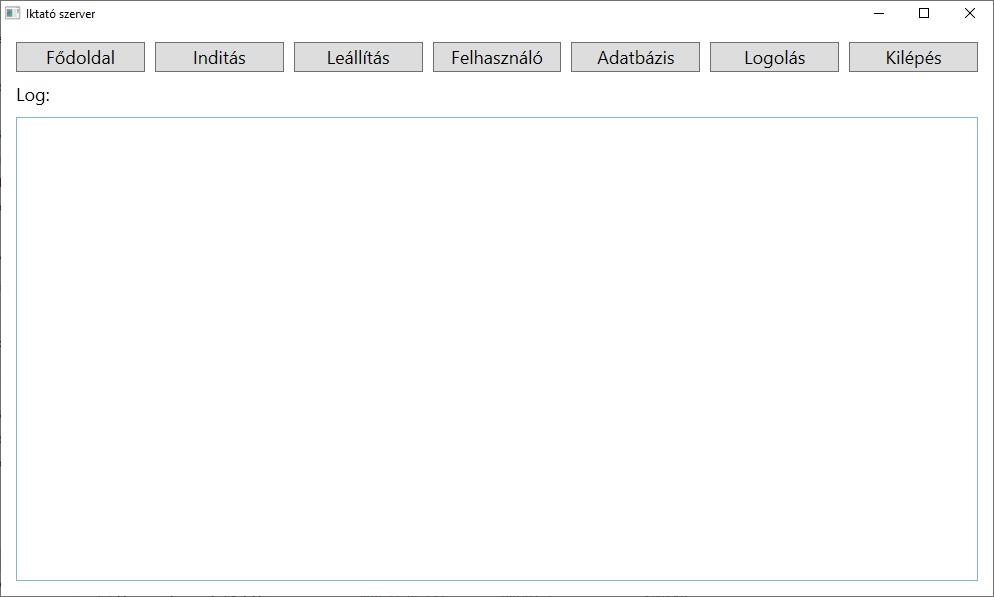
\includegraphics[width=7cm]{dokukepek/sfooldal}
	\caption{Szerver főoldala.}
	\label{fig:sfooldal}
\end{figure}

A szerver telepítésekor nem sok tenni valónk van mint, a kapott állományokat rá tesszük a számítógépünkre. Miután ez megtörtént a konfigurációs állományba módosítást kell végezni(IktatogRPCServer.exe.config) ahová beleírjuk a következő adatokat, 
\begin{itemize}
	\item[] APPHOST: Ami azt jelzi a programnak, hogy milyen ip címen fog ő működni.
	\item[] APPPORT: Azt jelzi a program számára, hogy milyen porton kell figyelnie.
	\item[] Secure: Azt jelzi a program számára, hogy milyen csatornát fog használni a kliens és szerver közötti kommunikáció során. Ha az érték "true" akkor szükség van először generálni egy kulcs párt, és azt hozzáadni a szerver certs mappájába. server.crt és server.key néven. Ha "false" akkor nincs szükség ezekre a fájlokra, mert titkosítatlan csatornát fognak használni.(Ezt a kliensen is be kell állítani).
	\item[] Test: Ide kell beírnunk az adatbázis connectionstringjét.(MySQL-re van szükség)
\end{itemize}

Ha ez megtörént elindíthatjuk a szervert az IktatogRPCServer.exe fájl segítségével. Ezután a következő kép fog fogadni minket:

Még mielőtt rá megyünk az indítás gombra be kell töltenünk az alap adatbázis csomagot, amit az "Adatbázis" fülön tudunk megtenni. Miután rákattintottunk, két lehetőséget fogunk látni, adatbázis mentése és visszatöltése.(\Az{\ref{fig:sadat}} ábra) Nekünk most a visszatöltés fog kelleni.
\begin{figure}[h!]
	\centering
	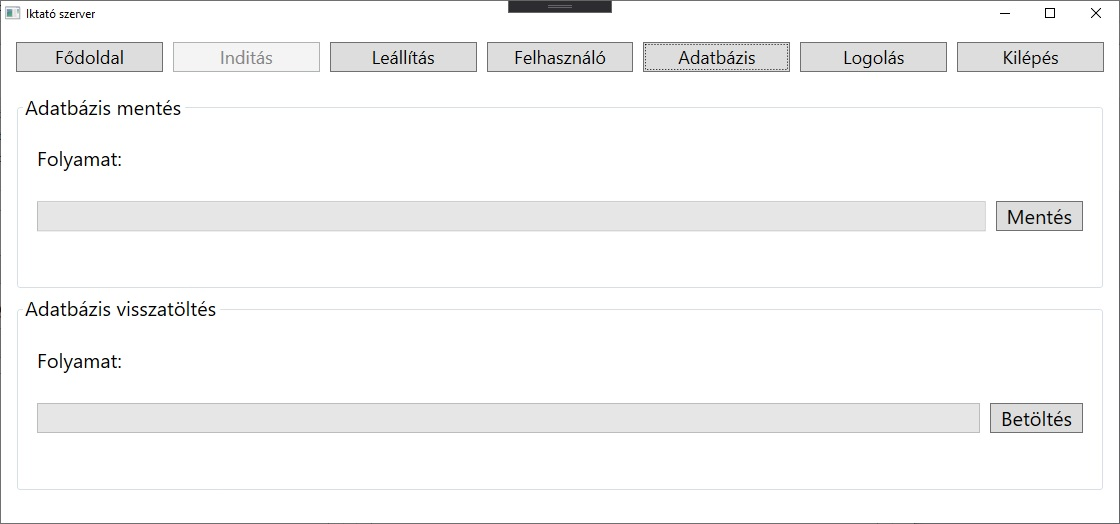
\includegraphics[width=7cm]{dokukepek/sadat}
	\caption{Adatbázis műveletek}
	\label{fig:sadat}
\end{figure}
Rákattintunk a betöltés gombra és meg fog jelenni egy fájl kiválasztó itt megkeressük az üres adatbázis scriptet vagy a demo adatbázist töltjük be. Ha a demot választjuk akkor a bejelentkezési lehetőség a következő. Felhasználónév: noname Jelszó: 12345678.(Ilyenkor lehet ugrani a kliens bemutatásra.) Én most a szerint írom tovább a telepítést mintha az üreset töltöttük volna be. Miután sikeresen betöltötte a scriptet létre kell hoznunk egy alap felhasználót a kliensek számára, ez a felhasználó fog majd tudni felvenni az elején telephelyeket, új felhasználókat stb\dots. (\Az{\ref{fig:sfelh} ábra}) Ha átváltottunk a felhasználó menüre akkor létre hozunk egy új felhasználót, ennek a felhasználónak megadjuk a felhasználónevét(min 4 karakter), teljes nevét(szóközt tartalmaznia kell), jelszavát(min 5 karakter) és kiválasztjuk, hogy ő admin lesz ezáltal nem szükséges megadnunk telephelyet, mivel később ő a kliensen belül magához tudja rendelni azt.
\begin{figure}[!h]
	\centering
	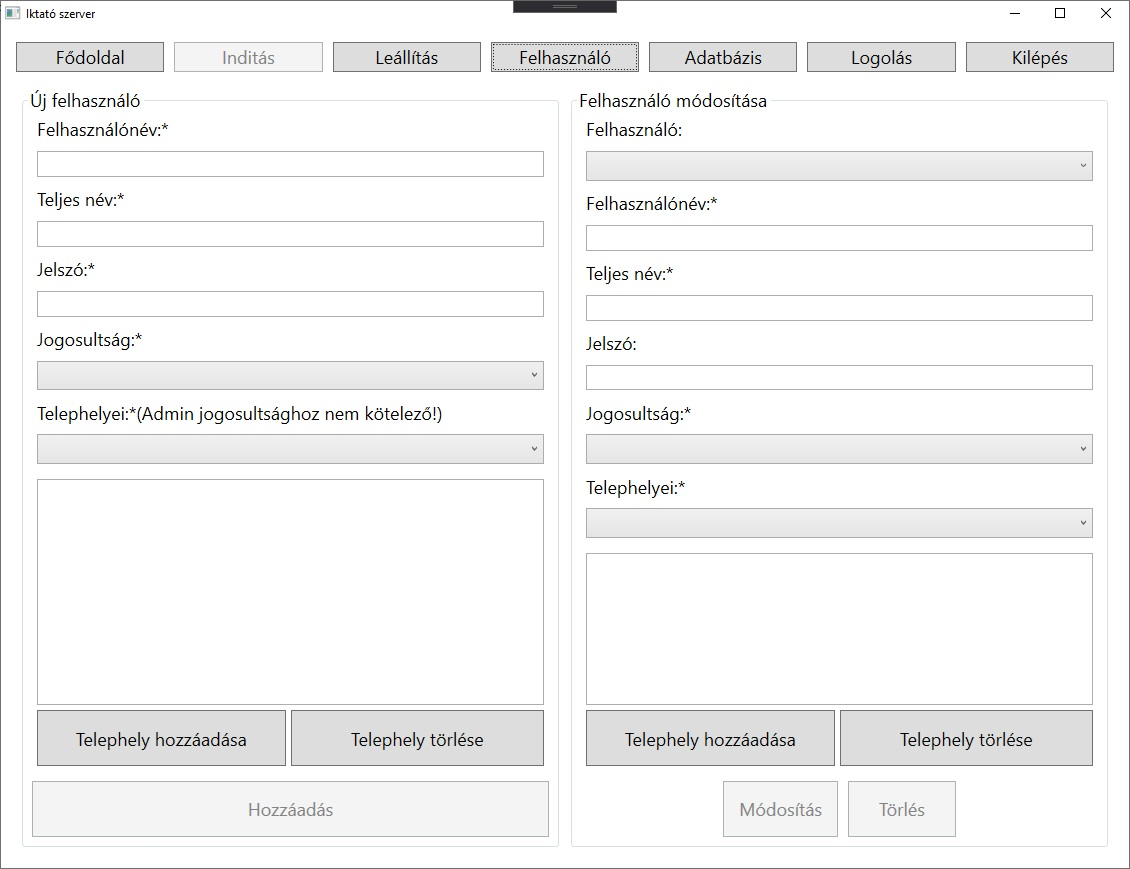
\includegraphics[height=7cm]{dokukepek/sfelh}
	\caption{Alap felhasználó hozzáadása}
	\label{fig:sfelh}
\end{figure}
Itt van lehetőségünk még felhasználó módosítására is. Illetve itt található meg a jelszó módosítás opció is. Ezután vissza mehetünk a főoldalra és elindíthatjuk a szervert.
\begin{figure}[!h]
	\centering
	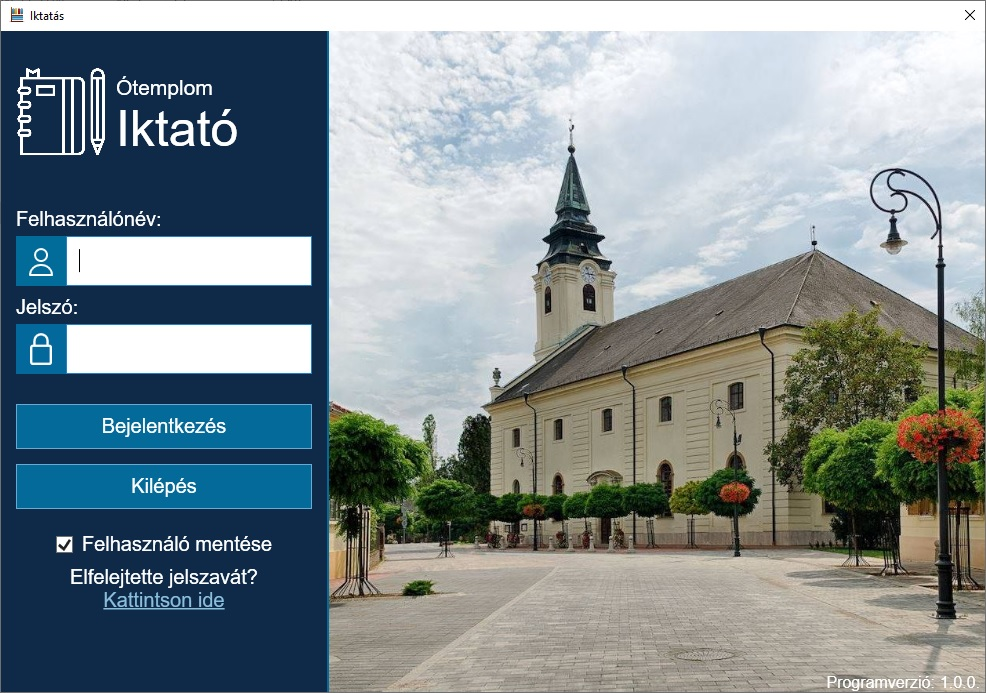
\includegraphics[width=7cm]{dokukepek/clogin}
	\caption{Bejelentkezés a szerveren hozzáadott felhasználóval.}
	\label{fig:clogin}
\end{figure} 
Most már van lehetőségünk a kliensen bejelentkezni. A bejelentkezéskor előtt a kliensen is módosítani kell a konfigurációs állományt az előzőekben leírt módon. 
Ha az megtörtént az előbb létre hozott felhasználóval be is tudunk jelentkezni. Sikertelen bejelentkezés esetén a rendszer kiírja a hibát, ha a szerver nem elérhető hibát kapjuk valószínűleg nem egyeznek meg a konfigurációs állományok a szerverrel. A használathoz először a törzs-be kell belemennünk és hozzá kell adunk egy telephelyet. Ne lepődjünk meg, hogy nem látjuk a hozzáadott telephelyet, mert után hozzá kell adni a felhasználó számára is, úgy hogy módosítjuk azt. Módosításkor a "Telephelyei" legördülő menüjében megjelenik az új telephely. Adjuk hozzá a felhasználónkhoz, ezután rá kattinthatunk a módosítás gombra. Majd újra lekérjük a törzs menü pontot és már látszódik is a telephely. Ugyan ilyen módon több telephelyet is hozzáadhatunk. Ha ezzel végeztünk létre hozhatjuk a többi felhasználókat és adatokat.
\section{Felhasználói dokumentáció}
\subsection{Bejelentkezés}
\begin{figure}[!ht]
	\centering
	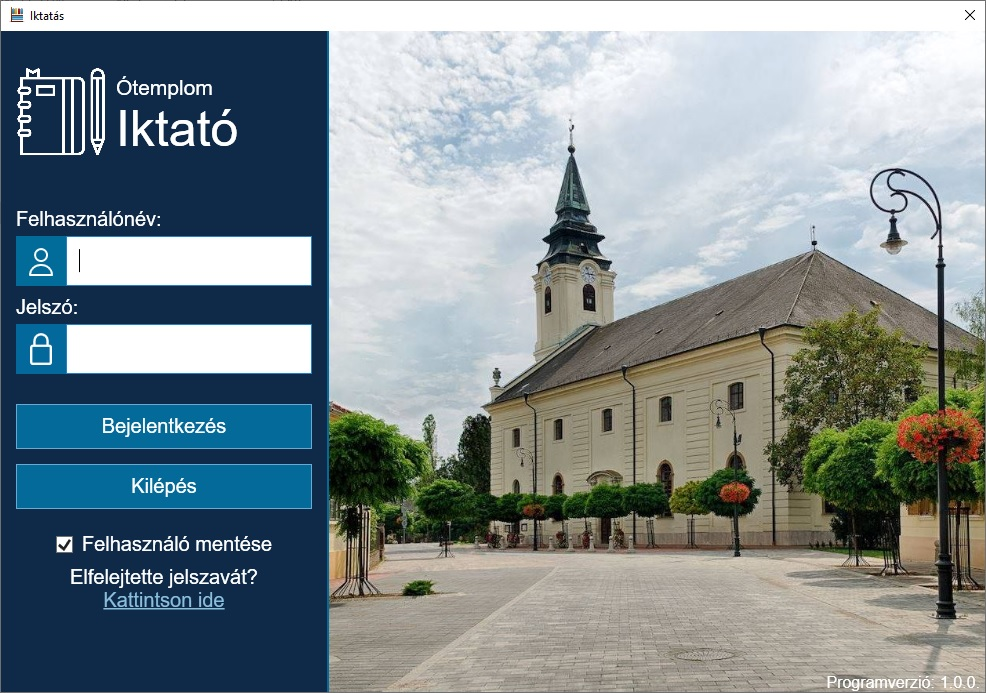
\includegraphics[width=7cm]{dokukepek/clogin}
	\caption{Bejelentkezés ablak.}
	\label{fig:clogin2}
\end{figure}
A bejelentkezéshez nem kell mást tennünk, mint beírjuk a kapott felhasználó és jelszó párost. A bejelentkezésnél van még lehetőség a felhasználónevünk elmentésére ha kipipáljuk a kis jelölő négyzetet. Így ha legközelebb elindítjuk a programot akkor már ezt nem fog kelleni beírni újra. Felhasználót a rendszergazdától vagy vezetőségtől lehet kérni. Ha elfelejtette a jelszavát egyenlőre még a rendszergazdát kell keresnie, de a későbbiekben használható lesz az "elfelejtett jelszó" funkció is.
\subsection{Törzs}
A törzs menüben tudja kezelni az iktatáshoz szükséges adatokat, mint például Ügyintézők, Jellegek, Partnerek, Partnerek ügyintézői stb\dots Mindegyik fajtának találhatunk egy kis ablakot. \Az{\ref{fig:ctorzs}} ábrán látható. Mindegyik ablakban van hozzáadás, módosítás és törlési lehetőség. Viszont vannak olyan lehetőségek, amiket csak admin jogosultsággal rendelkező felhasználó tud kezelni. Mint az év, csoportok, telephelyek, felhasználók. Így ők tudnak felhasználót is felvinni, telephelyeket hozzáadni, elvenni felhasználóktól és évet zárni. 
\begin{figure}[h!]
	\centering
	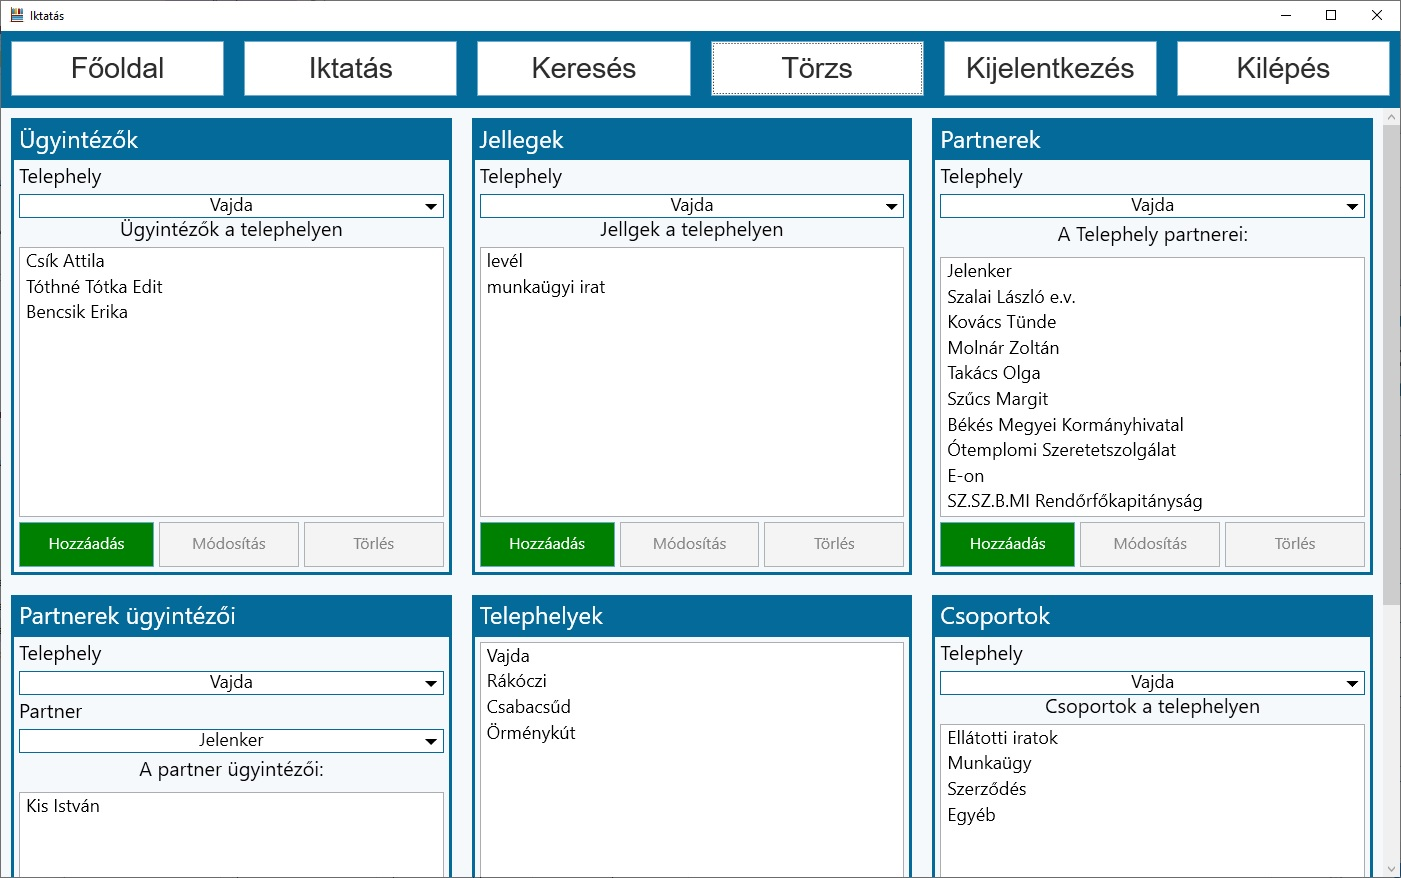
\includegraphics[width=7cm]{dokukepek/ctorzs}
	\caption{}
	\label{fig:ctorzs}
\end{figure}
\textbf{Példa hozzáadás:}
Miután rákattintottunk az ügyintézőknél a hozzáadás gombra van lehetőségünk telephelyet kiválasztani és új nevet beírni. Ha ezt megtettük és az adatokat helyesek a felvitelhez(nem üres és nagyobb mint 5 és kisebb mint 50 hosszú) akkor a hozzáadás gomb zöldre vált. Ha rákattintottunk, akkor hozzáadja az új ügyintézőt az adatbázishoz és vissza lép a lista nézetbe. \\
\textbf{Példa módosítást:}
\begin{figure}[h!]
	\centering
	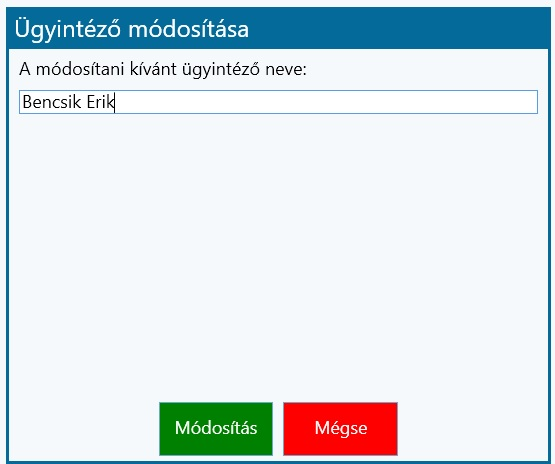
\includegraphics[width=7cm]{dokukepek/ctorzsmod}
	\caption{Ügyintéző módosítása}
	\label{fig:ctorzsmod}
\end{figure}
A módosításhoz ki kell jelölnünk a módosítani kívánt személyt , ha ez megtörtént a módosítás gomb zöldre vált és a következő nézetben láthatjuk az ügyintéző módosítható adatait. Ha módosítottuk az adatot és megfelel az adat felvitel kritériumainak(nem üres és nagyobb mint 5 és kisebb mint 50 hosszú) akkor a módosítás gomb zöldre vált. Ha rákattintottunk, akkor módosítja az ügyintézőt az adatbázisban és vissza lép a lista nézetbe.\\
\textbf{Példa törlés:}
A törlés mindegyik lehetőségnél ugyan úgy működik. Ha kijelöljük a törölni kívánt adatot akkor az ablakon a törlés gomb pirosra vált és ha megnyomjuk akkor ki is törli az adatbázisból és a listánkból is.
\begin{figure}[h!]
	\centering
	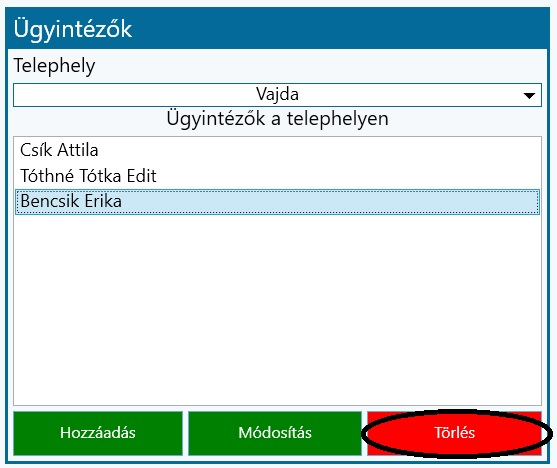
\includegraphics[width=7cm]{dokukepek/ctorzsdelete}
	\caption{Ügyintéző törlése}
	\label{fig:ctorzsdelete}
\end{figure}
\subsection{Iktatás}
\begin{figure}[h!]
	\centering
	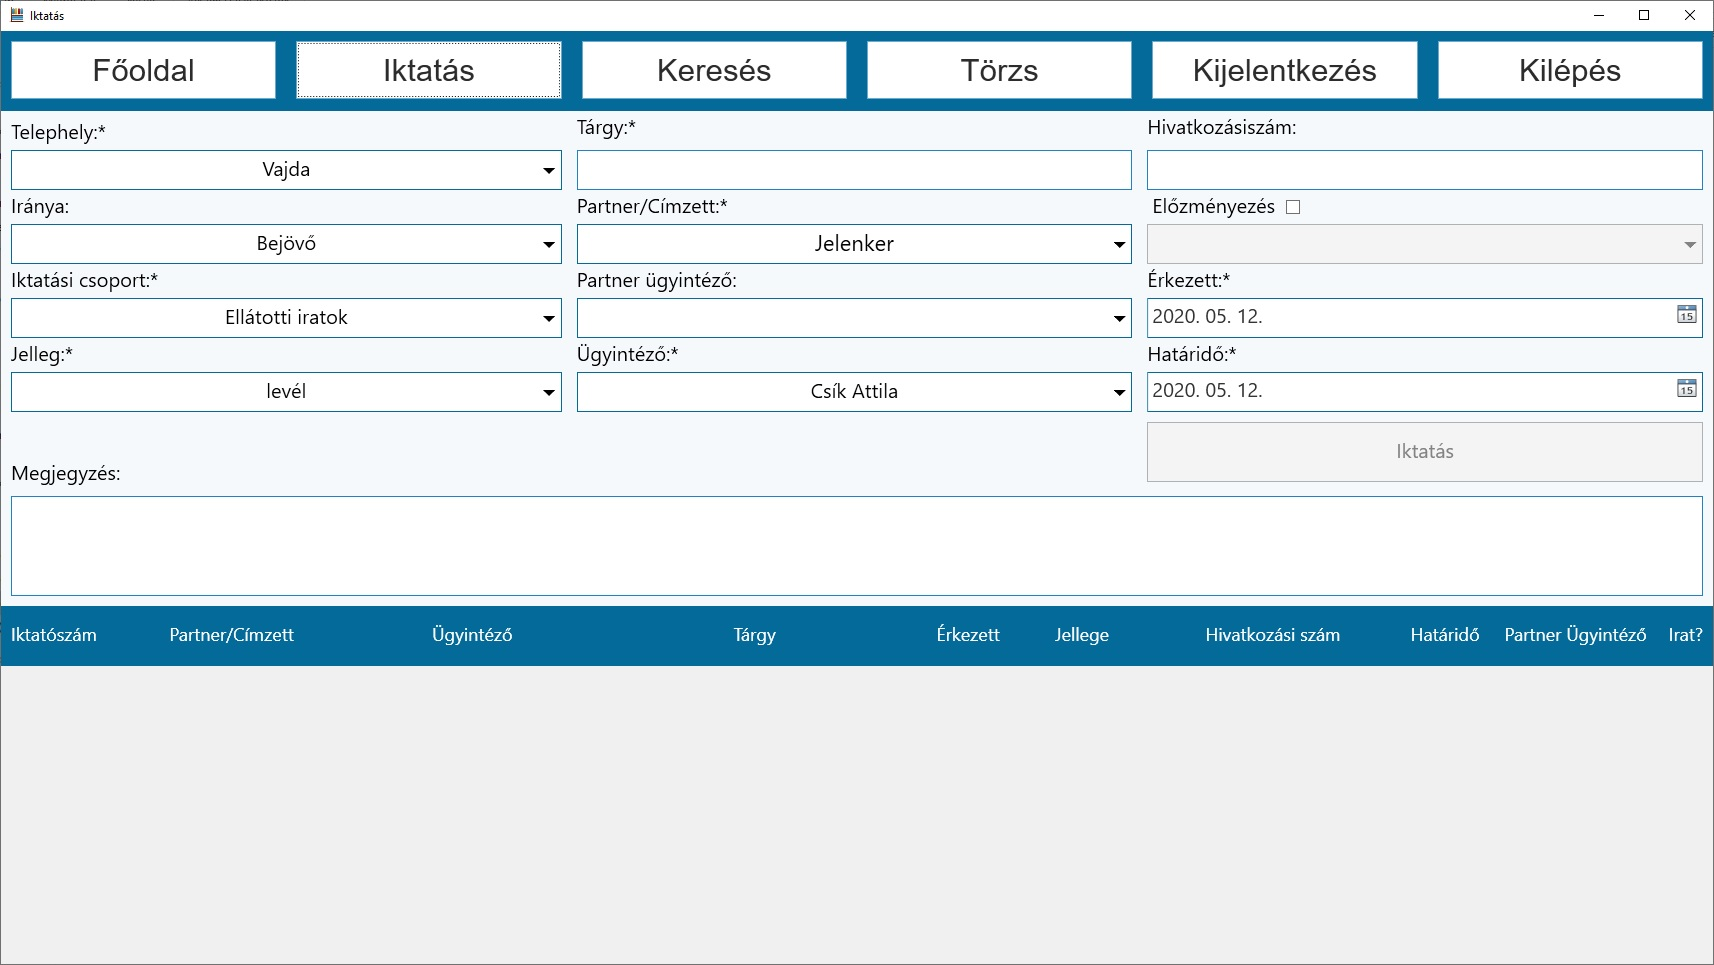
\includegraphics[width=7cm]{dokukepek/ciktatas}
	\caption{Iktatás hozzáadása}
	\label{fig:ciktatas}
\end{figure}
Az iktatásnál majdnem minden mező kitöltése kötelező. Kivéve a megjegyzés, a hivatkozási szám, partner ügyintéző és az előzményezés. Ha ezeken kívül mindent kitöltünk és a tárgy karakter hosszúsága is legalább 3 és maximum 100 között van akkor az iktatás gomb kékre vált. Ha rákattintunk az adatbázisba mentés után megkapjuk az iktató számunkat amit egy felugró ablak segítségével jelenít meg számunkra a program. Ezután még hozzáadja a nemrégiben hozzáadott iktatások listájához is. Ez a lista csak a program újra indításakor vagy kijelentkezéskor törlődik.
\subsection{Keresés}
\begin{figure}[h!]
	\centering
	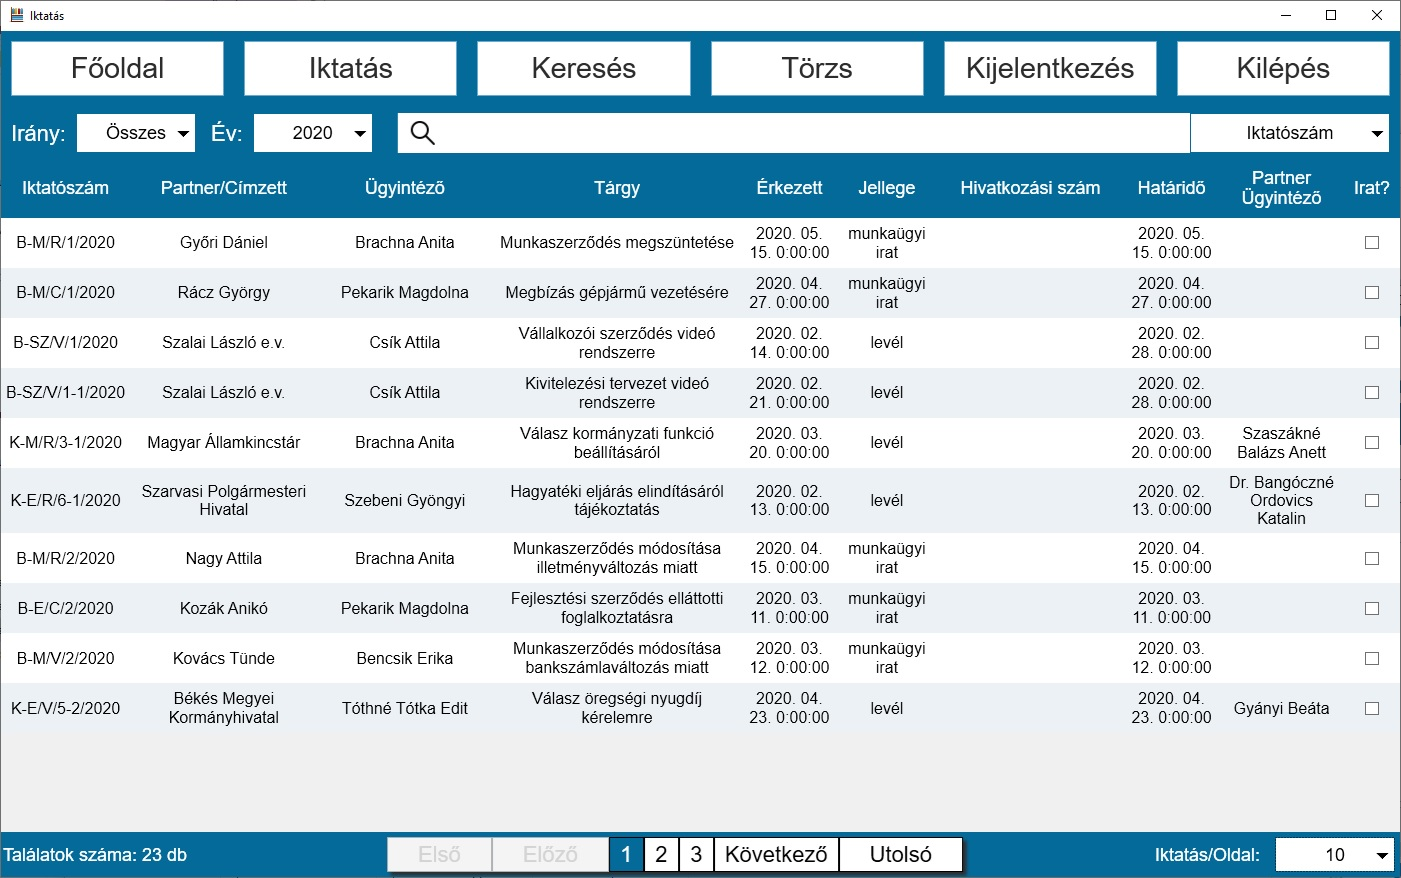
\includegraphics[width=7cm]{dokukepek/ckereses}
	\caption{Keresés}
	\label{fig:ckereses}
\end{figure}
A keresés legelső fázisa az, hogy megadjuk az iktatás irányát és az évét. Ezután a program el is kezdi leszedni a dokumentumokat. Miután leszedte megjelenít annyit belőle amennyit az "Iktatás/Oldal" szám mutat. Ezt is tudjuk módosítani ilyenkor automatikusan újra generálja a megjelenített nézetett. Ha szűrni szeretnénk akkor a lista feletti kereső sávban ezt megtehetjük. A szűrési feltétel kiválasztása után Pl.: Iktatószám kijelölésével van lehetőségünk iktatószámra keresni. Ilyenkor amit a kereső sávba beírtunk szövegre illeszkedő iktatásokat fogja megjeleníteni.
\subsection{Iktatás módosítás}
Ha a keresésben vagy az iktatás fülön az iktatás listájában valamelyik dokumentumra kétszer rákattintunk akkor lesz lehetőségünk az iktatás módosítására.
\begin{figure}[h!]
	\centering
	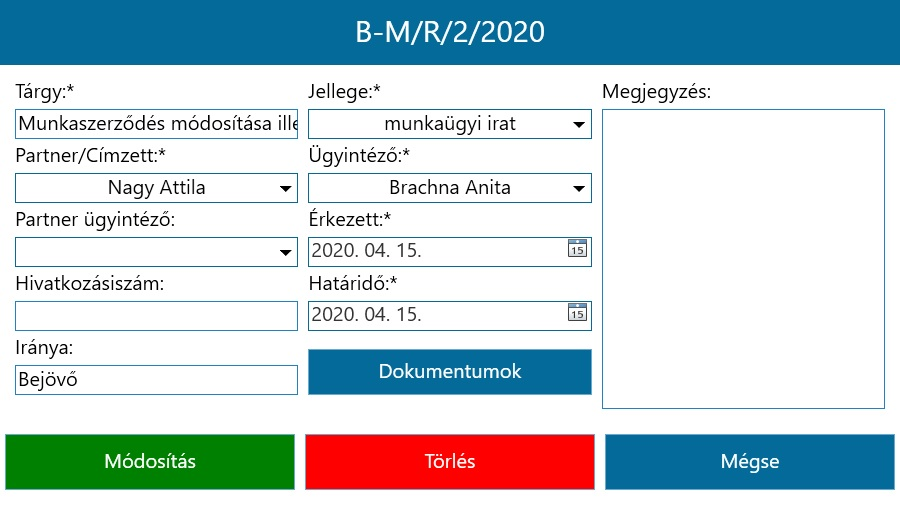
\includegraphics[width=7cm]{dokukepek/ciktatmod}
	\caption{Iktatás módosítása}
	\label{fig:ciktatmod}
\end{figure}
Módosítani csak azokat a mezőket tudjuk amik nem befolyásolják az iktató számot. Az ablak tetején láthatjuk a kiválasztott iktatás számát, ezzel is biztosítjuk a felhasználót, hogy jó iktatást akar módosítani. Ha minden mező megfelel a kritériumoknak (ugyan az mint iktatáskor) akkor a Módosítás gomb zöld marad/lesz. Miután rámegyünk a módosításra az a listában is frissíteni fogja az iktatást, nem kell újra lekérdezni azokat.
\subsection{Dokumentumkezelés}
A dokumentumok kezelését is a módosítás fülön érjük el. Ha rákattintunk a Dokumentumok gombra akkor fog megjelenni az iktatáshoz feltöltött anyagok listája. Illetve itt van még lehetőségünk a dokumentumok feltöltésére, letöltésére és törlésére.
\subsubsection{Feltöltés}
\begin{figure}[h!]
	\centering
	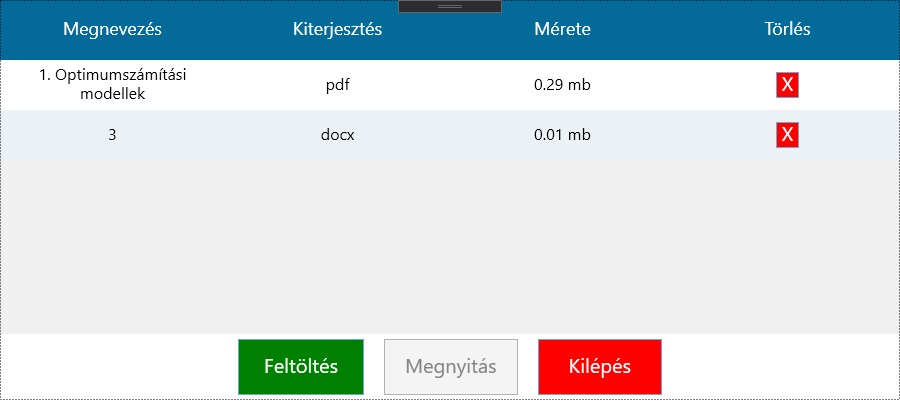
\includegraphics[width=7cm]{dokukepek/cfeltoltes}
	\caption{Feltöltés}
	\label{fig:cfeltoltes}
\end{figure}
Dokumentum feltöltése nagyon egyszerű feladat. Egyszerűen rámegyünk a feltöltés gombra ahol utána egy fájl kiválasztó ablak fog megjelenni. Egyszerre csak egy elemet lehet feltölteni és csak a következő típusúakat DOCX, DOC, XLS, XLSX, PDF. Miután kiválasztottuk a fájlunkat meg is indul a feltöltés. Feltöltés után megjelenik a feltöltött dokumentum, ahol már látjuk is a nevét, kiterjesztését, méretét. 
\subsubsection{Letöltés}
\begin{figure}[h!]
	\centering
	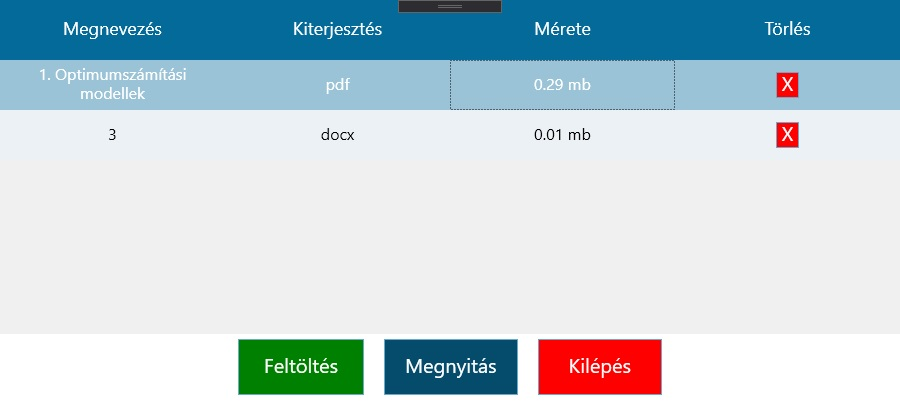
\includegraphics[width=7cm]{dokukepek/cletoltes}
	\caption{Letöltés}
	\label{fig:cletoltes}
\end{figure}
A letöltés megegyezik a megnyitással miután kijelöltük a letölteni kívánt dokumentumot(egyszer rákattintunk) akkor a megnyitás gomb kékre változik, ha ezután rá kattintunk akkor megindul a dokumentum letöltése és megnyitása. Minden dokumentumot a kiterjesztésnek megfelelő alapértelmezett programmal nyitja meg, ha erre nincs lehetősége hibát fog dobni a program. Miután megnyitottuk a dokumentumot lesz lehetőségünk menteni másként azt.
\subsection{Kijelentkezés$\backslash$Kilépés}
A kilépés és a kijelentkezés is a menüsorban található meg, mind a kettő kijelentkezteti a szerverről először a felhasználót. Viszont utána a kijelentkezés gomb újra megjeleníti nekünk a bejelentkezési felületet, a kilépés viszont bezárja a programot.
\chapter{Továbbfejlesztési lehetőségek}
A programot lassan egy hónapja használják. Ez alapján kapott visszajelzések azt mutatják, hogy követelmény specifikációban leírtak teljesen lefedték a mindennapi használat során felmerülő funkciókat. Kisebb tovább fejlesztésekre tartanak igényt, mint például az új iktatáskor a tárgy illetve hivatkozási szám mezőben legyen automatikus kitöltési lehetőség, azaz előzőleg felvitt iktatások adataiból lehessen választani. Ez nagyban lecsökkentené a felvitelre szánt időt a program felhasználói számára. 

Sajnálatos módon már nem volt időm a következő feladatokra, amiket még terveztem a program készítése során, de a jövőben fejlesztésre kerülnek:
\begin{itemize}[leftmargin=0pt]
	\item \underline{\textit{Mentés ütemezés: }}A szerver oldalra terveztem egy olyan funkciót, ahol be lehet állítani, hogy az adatbázisról milyen időközökként készítsen mentést és azt hova helyezze a merevlemezen. Ez által is csökkentve a szerver adminisztrátor terhét. Ebből a funkcióból egyelőre csak az adatbázis mentése funkció került megvalósításra. 
	\item \underline{\textit{Cache/Cache kezelés: }}Az adatbázis szerver felé irányuló folyamatokat szeretném ezáltal csökkenteni. Egy proxy osztályt fogok létrehozni az adatbázis kezelő osztályokból, így azok el fogják tárolni a lekért adatokat, és ha nem volt módosítás a következő kéréskor, akkor ők azt fogják visszaadni. Ezeknek az osztályoknak a kezelését is elérhetővé fogom tenni a szerver oldalon, azaz ha túl nagy lenne egy cache, akkor onnan könnyen lehet majd azokat törölni.
	\item \underline{\textit{Csoportosítás: }}A kliens oldalon lévő keresés menüpontnál lévő datagrid-ben az iktatások csoportosítása előzményezés szerint. Azaz ha egy iktatószámnak vannak „gyermekei” akkor az a „szülő” melletti + gomb által lesznek megjeleníthetőek, lenyithatóak. 
	\item \underline{\textit{Hiba kezelés bővítése: }}A kliensben pontosabb hibaüzenetek létrehozása adatfelvitelkor. Így a felhasználó sem fog kérdésekbe bocsátkozni még akkor is, ha a hiba mivolta teljesen egyértelmű.
	\item \underline{\textit{Elfelejtett jelszó: }}A bejelentkezésnél található az elfelejtett jelszó link, erre se volt sajnos időm. A megvalósítása valószínűleg úgy lesz, hogy küld a felhasználó e-mail címére egy kódot(később email is fog kelleni felhasználó létrehozáshoz) és a kód beírásával előjön a jelszó módosítás ablak.
\end{itemize}
\chapter{Összefoglalás}
A szakdolgozatom kitűzött célja az volt, hogy az Ótemplomi Szeretetszolgálat jelenlegi ügyviteli rendszerét lecseréljem. A jelenlegi helyzetben lévő problémák az iktatással kapcsolatban, hogy a bevezetésben említett egyesülés után az Excel dokumentumok száma megnövekedett. Az iktatáshoz használt munkafüzetek hátránya, hogy az iktatások konzisztenciájának megőrzése lehetetlen, azaz egy-egy be-és kimenő irat is kaphat olyan számot, ami már foglalt, illetve előfordulnak, olyan esetek, amelyek több munkacsoportot is érintenek, emiatt egy iktatást többször vagy egyszer sem iktatnak le. Az iktatásokhoz nem lehet előzményezést rendelni. Az iktatott dokumentumokat csak több perces keresés árán tudják megtalálni. A gazdasági vezető nem képes nyomon követni telephelyek iktatásait, illetve bármilyen dokumentumot elérni.  Valamint probléma, hogy a dokumentumokról nem készül semmilyen mentés, archiválás.

Ezekre a hibákra az iktatóprogram fejlesztése hozott megoldást. Most már központosítottá vált. A vezető által kért nyomon követési lehetőség elérhető lett. Mindenki az iktatást egy kliens segítségével éri el, bejelentkezés után. Ezáltal naplózhatóvá vált, hogy ki, mit csinál a rendszerben. Az iktatószám generálását most már a szerver látja el, ezáltal kiküszöböltük a számok többszöri kiadását. Egy átláthatóbb felületet kaptunk az iktatás felvitelére, keresésére és a törzsadatok kezelésére.  A felvitelkor a már tárolt törzsadatok biztosítják a pontos, precíz adatok kitöltését, illetve egyes felhasználók több telehelyhez is rögzíthetnek iktatást.  A kereséskor csak a legfontosabb adatokat jelenítjük meg. Elérhetővé vált a paraméteres keresés és szűrés.  Az iktatásokhoz megvalósult a kapcsolódó dokumentumok egy helyen való kezelése is, így most már egyszerűbb ezen adatok megtekintése, feltöltése és letöltése. 

A szerver oldal elérhetővé tette számunkra az adatbázis mentését, és annak archiválását. A felhasználók egyhelyen való kezelését. Ahol az adminisztrátor hozzárendelhet, illetve eltávolíthat telephelyeket a userektől. Ezt a lehetőséget admin jogosultsággal rendelkező felhasználó is eléri a kliens oldalról, viszont jelszó módosításra csak itt van lehetőség.  A logolás helyét és szintjét is beállíthatjuk. A szint alapértelmezetten warningon van, azaz csak olyan hibák fognak mentésre kerülni, amik nagyban befolyásolják a program működését. Ha a klienst paraméteresen (-d) indítjuk akkor az automatikusan debug módra vált. A szerver és a kliens között ez TLS kapcsolat van SSL titkosítással. 

Az eddigi tapasztaltak alapján a kollégák nagy örömmel fogadták a programot. Kaptam tovább fejlesztésre való ötleteket illetve kisebb javítási igényeket a felhasználó felületben.  Úgy érzem, a gazdasági vezető által kitűzött, és a felhasználók munka végezésének megkönnyítésére tett célokat elértük.
\begin{thebibliography}{2}
\bibitem{excel}
\textsc{Excel: }https://www.forbes.com/sites/bernardmarr/2016/06/16/spreadsheet-reporting-5-reasons-why-it-is-bad-for-business/	
\bibitem{mvvmmicrosoft} \textsc{MVVM:} https://docs.microsoft.com/en-us/previous-versions/msp-n-p/hh848246(v=pandp.10)
\bibitem{torveny}
\textsc{Törvény}:https://net.jogtar.hu/jogszabaly?docid=99500066.TV
\bibitem{rendelet}
\textsc{Kormány rendelet}: https://net.jogtar.hu/jogszabaly?docid=A0500335.
KOR\&searchUrl=/gyorskereso\%3Fkeyword\%3D335/2005.\%2520
\bibitem{mvvmbook}
\textsc{MVVM könyv: } MVVM Survival Guide for Enterprise Architectures in Silverlight and WPF
\bibitem{caliburn}\textsc{Caliburn.Micro: }https://caliburnmicro.com/
\bibitem{grpc}\textsc{gRPC: }https://grpc.io/docs/guides/
\bibitem{grpcprotokol}
\textsc{Protokoll: } https://blog.container-solutions.com/introduction-to-grpc
\bibitem{openssl}
\textsc{SSL:} https://bbengfort.github.io/programmer/2017/03/03/secure-grpc.html
\bibitem{channel}
\textsc{gRPC Csatorna: } https://github.com/grpc/grpc/issues/16038
\bibitem{serverauth}
\textsc{Szerver módok:} https://grpc.io/docs/guides/auth/
\bibitem{errorhandling}
\textsc{Hibakezelés:} https://docs.microsoft.com/en-us/dotnet/architecture/grpc-for-wcf-developers/error-handling


\end{thebibliography}


\end{document}